\chapter{Geometric Modeling of Discrete Data} \label{ch:simplex}

In this chapter we propose using the Aitchison geometry of the simplex space for modeling discrete data. The main idea is to represent simplex-valued distributions in Euclidean coordinates in a way that respects their natural geometry. We consider two applications of this idea: generative modeling of discrete data (Paper~III) and Gaussian process classification (Paper~IV).

We first introduce the Aitchison geometry and the simplex-to-Euclidean bijections that are used through the chapter. We then present stochastic interpolations that move discrete data from the boundary of the simplex to the interior, and provide theoretical guarantees for the recovery of the original discrete values. In the interior of the space we can use the bijections for modeling continuously in Euclidean coordinates, making the modeling compatible with Euclidean continuous methods. These ingredients are combined in two case studies: Simplex-to-Euclidean Flow Matching for generation of discrete data and Isometric Logratio Gaussian Processes for multiclass classification.


\paragraph{Motivation} We find that the Aitchison geometry provides for the  simplex, a geometry-aware representation that, combined with the stochastic interpolations, connects discrete modeling to known Euclidean methods. This makes existing Euclidean methods applicable to these tasks (generation and classification), providing a unified modeling framework that is exact and compatible with state-of-the-art Euclidean models while respecting the geometry of log proportions.

\section{Simplex-to-Euclidean Bijections}

We presented in Section~\ref{sec:discrete_data} the Fisher information geometry in the simplex, which is isomorphic to the positive orthant of the sphere. In this section and through the chapter, we instead use the Aitchison geometry of the simplex, because it provides a direct connection between the open simplex and Euclidean coordinates. We now introduce compositional data analysis which provides the building blocks for the Simplex-to-Euclidean bijections.

\subsection{Compositional Data Analysis}

\citet{Aitchison1981, Aitchison1982} introduced a geometry for the simplex that is not the Fisher information metric. This geometry is defined only on the interior of the simplex and the central idea is that information is carried by  the log-ratios of the components. Similarly to how the sigmoid function is a link function from binary classification to $\mathbb{R}$, the Aitchison geometry gives different choices of link functions from the open simplex to $\mathbb{R}^D$. The bijections make Euclidean modeling compatible with the simplex.

\paragraph{The geometry of the simplex}
Consider $K$-class categorical data $c\in\{1,\dots,K\}$, let $D:=K-1$.
The simplex and the open simplex are defined as
\begin{equation*}
    \Delta^{D}:=\{\boldsymbol{x}\in\mathbb{R}_{\ge 0}^{K}:\;\sum_{k=1}^{K}x_k=1\}, \quad 
    \mathring{\Delta}^{D}:=\{\boldsymbol{x}\in\mathbb{R}_{> 0}^{K}:\;\sum_{k=1}^{K}x_k=1\},
\end{equation*}
where only $D=K-1$ components are free, since one arbitrary component (for example the last one) is determined by the others as $x_K = 1-\sum_{d=1}^D x_d$.
The usual Euclidean operators are not closed on the simplex, for example the Euclidean sum of two vectors may fall outside the space. For this reason, \cite{Aitchison1986} defines perturbation (vector addition) and powering (scalar multiplication) that make the simplex a vector space. Define the normalization operation $\mathcal{C}(\boldsymbol{x}) := \boldsymbol{x}/\sum_{k=1}^{K} x_k$. For $\boldsymbol{x}, \boldsymbol{y}\in\mathring\Delta^D$ and $\lambda\in \mathbb{R}$, define
\begin{align*}
\textbf{perturbation} \quad
&\boldsymbol{x} \oplus \boldsymbol{y}
:= \mathcal{C}(x_1 y_1,\ldots, x_K y_K), \text{ and} \\
\textbf{powering} \quad
&\lambda \odot \boldsymbol{x}
:= \mathcal{C}(x_1^\lambda,\ldots, x_K^\lambda).
\end{align*}
Under these operations, $(\mathring\Delta^D, \oplus, \odot)$ is a vector space and the neutral element  is $\tfrac{1}{K}\boldsymbol{1}$ since $\boldsymbol x \oplus (\tfrac{1}{K}\boldsymbol{1}) = \boldsymbol x$. The vector space is an inner product space when given the Aitchison inner product defined as
\begin{equation*}
\langle \boldsymbol{x}, \boldsymbol{y} \rangle_A := \frac{1}{2K} \sum_{i,j=1}^{K} 
\log\frac{x_i}{x_j}\log\frac{y_i}{y_j}.
\end{equation*}
The norm of a vector is $\|\boldsymbol{x}\|_A = \sqrt{\langle \boldsymbol{x}, \boldsymbol{x} \rangle_A}$. The distance between two compositions is 
\begin{equation*}
    d_A(\boldsymbol x,\boldsymbol y) = 
    \|\boldsymbol{x} \ominus \boldsymbol{y}\|_A
= \sqrt{\frac{1}{2K}\sum_{i,j=1}^K
\left(\log\frac{x_i}{x_j}-\log\frac{y_i}{y_j}\right)^2 },
\end{equation*}
where $\boldsymbol{x} \ominus \boldsymbol{y} :=  \boldsymbol{x} \oplus  (-1 \odot\boldsymbol{y})$.

\paragraph{The simplex as embedded  Riemannian manifold}
The simplex can be viewed as an embedded manifold in $\mathbb{R}^K$. It is the intersection of the hyperplane $\sum_{k=1}^K x_k=1$ and the positive orthant. Because the hyperplane is flat, all tangent spaces are parallel and identified with the zero-sum linear space
\begin{equation*}
\mathbb{H}^{D}=\left\{\boldsymbol{z}\in\mathbb{R}^K:\sum_{i=1}^K z_i=0\right\}.
\end{equation*}
To give the open simplex a geometry, we use the center logratio map (CLR), which is a bijection between  $\mathring \Delta^D$ and the zero-sum hyperplane $\mathbb{H}^D$
\begin{equation*}
\begin{aligned}
    \operatorname{clr}: \mathring\Delta^D &\to \mathbb{H}^D, \quad
    \boldsymbol{x} \mapsto \boldsymbol{z}
    = \log \boldsymbol{x} - \frac{1}{K}\sum_{k=1}^{K} \log x_k \,\boldsymbol{1}, \text{ and} \\
    \operatorname{clr}^{-1}: \mathbb{H}^D &\to \mathring\Delta^D, \quad
    \boldsymbol{z} \mapsto \boldsymbol{x}
    = \mathcal{C} (\exp\boldsymbol{z}).
\end{aligned}
\end{equation*}
The image of the map lies in $\mathbb{H}^{D}$ because the components of $\operatorname{clr}(\boldsymbol{x})$ sum to zero, and the inverse map is usually known as the \emph{softmax}. In addition, the center logratio map is an isometry between $(\mathring\Delta^{D},\langle\cdot,\cdot\rangle_A)$ and $(\mathbb{H}^{D},\langle\cdot,\cdot\rangle_2)$, since the Aitchison norm and inner products are (after some algebraic manipulations)
\begin{align*}
\langle \boldsymbol{x}, \boldsymbol{y} \rangle_A &= 
\langle \operatorname{clr}(\boldsymbol{x}), \operatorname{clr}(\boldsymbol{y}) \rangle_2 
=\frac{1}{2K} \sum_{i,j=1}^{K} 
\log\frac{x_i}{x_j}\log\frac{y_i}{y_j}, \text{ and} \\
d(x,y)_A &= 
\| \operatorname{clr}(\boldsymbol{x})- \operatorname{clr}(\boldsymbol{y}) \|_2 
 = \sqrt{\frac{1}{2K}\sum_{i,j=1}^K
\left(\log\frac{x_i}{x_j}-\log\frac{y_i}{y_j}\right)^2 }.
\end{align*}
This means that the Aitchison geometry of the simplex is inherited from $\mathbb{H}^{D}$ via the center logratio map, thus the Riemannian metric is the pullback metric:
\begin{equation*}
    \mathbf{G}(\boldsymbol{x}) = \mathbf{J}_{\mathrm{clr}}(\boldsymbol{x})^\top\mathbf{J}_{\mathrm{clr}}(\boldsymbol{x}),
\end{equation*}
for $\mathbf{J}_{\mathrm{clr}}(\boldsymbol{x}) = \pdv{\operatorname{clr}(\boldsymbol{x})}{\boldsymbol{x}_{1:D}}$ where the Jacobian is computed with respect to the first $D$ coordinates because of the extra degree of freedom and $x_K =1- \sum_{d=1}^Dx_d$. The geodesics are computed by pulling back straight lines in $\mathbb{H}^D$
\begin{equation*}
    \gamma(t) = \operatorname{clr}^{-1}\bigl((1-t)\operatorname{clr}(\boldsymbol{x}) + t\operatorname{clr}(\boldsymbol{y})\bigr) = 
    \bigl((1-t)\odot \boldsymbol{x}\bigr) \oplus \bigl(t\odot \boldsymbol{y}\bigr).
\end{equation*}


\paragraph{Isometric Logratio}
The CLR map gives the simplex the Aitchison geometry, but the image of the map still lands in the constrained hyperplane $\mathbb{H}^D$. For practical modeling it is more convenient to work in ordinary Euclidean coordinates. The isometric logratio (ILR) map of \citet{Egozcue2003} achieves this by expressing CLR coordinates in an orthonormal basis of $\mathbb{H}^D$. This basis is given by the Helmert matrix $\mathbf{H}\in \mathbb{R}^{D\times K}$ \citep{Lancaster1965}, and the resulting bijection is
\begin{equation*}
    \varphi(\boldsymbol{x}) = \mathbf{H} \, \operatorname{clr}(\boldsymbol{x}).
\end{equation*}
The Helmert matrix has the property that $\mathbf{H}\boldsymbol{1} = \boldsymbol{0}$, then 
\begin{equation*}
\mathbf{H} \, \operatorname{clr}(\boldsymbol{x})
=
\mathbf{H} \log \boldsymbol{x}
-
\frac{1}{K}\sum_{k=1}^{K} \log x_k \,
\underbrace{\mathbf{H}\boldsymbol{1}}_{=\boldsymbol{0}}
=
\mathbf{H} \log \boldsymbol{x}.
\end{equation*}
The ILR map and its inverse are therefore
\begin{equation} \label{eq:ilr}
    \begin{aligned}
    \varphi: \mathring\Delta^{D} \to \mathbb{R}^{D},\quad  &\boldsymbol{x}\mapsto \boldsymbol{z}= \mathbf{H} \log \boldsymbol{x}, \text{ and} \\
    \varphi^{-1}:  \mathbb{R}^{D} \to \mathring\Delta^{D}, \quad &\boldsymbol{z}\mapsto \boldsymbol{x} = \mathcal{C}\left(\exp (\mathbf{H}^\top \boldsymbol{z} )\right).
    \end{aligned}
\end{equation}
This bijection is simpler because we can use the standard basis of the Euclidean space $\mathbb{R}^D$ along with the Euclidean inner product to model in the latent space while preserving the Aitchison geometry. The isometry is stated in Theorem~\ref{thm:isometry}, and the proof is omitted here. A visualization of the Aitchison geometry is in Figure~\ref{fig:fig1}, which shows the latent distribution and geodesic balls on both spaces.
\begin{figure}
    \centering
    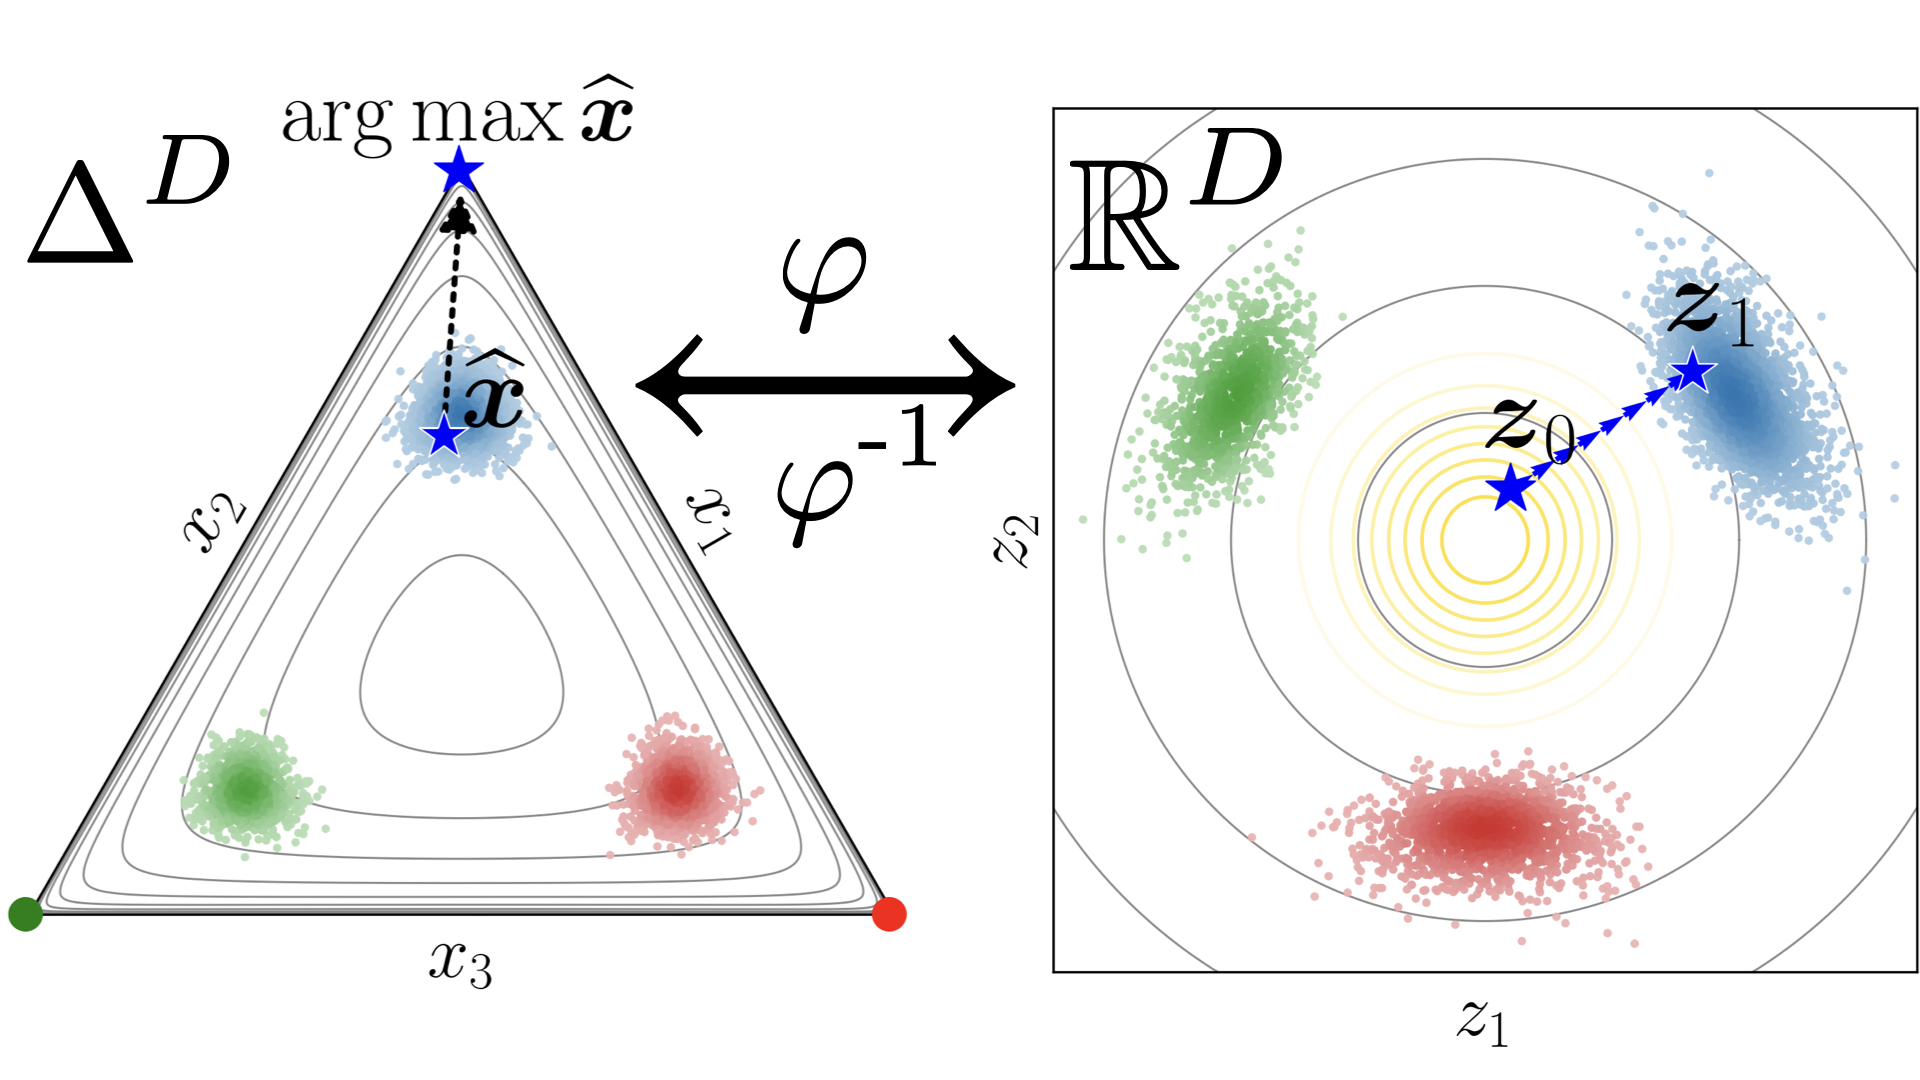
\includegraphics[width=0.8\linewidth]{figs/paper3/fig1.001.jpeg}
    \caption{Visual representation of the Aitchison geometry and Simplex-to-Euclidean Flow Matching.}
    \label{fig:fig1}
\end{figure}

\begin{theorem}[Isometry, \citep{Egozcue2003}]\label{thm:isometry}
Let $\langle\cdot,\cdot\rangle_A$ denote the Aitchison inner product on $\mathring \Delta^{D}$ and $\langle\cdot,\cdot\rangle_2$ the standard inner product on $\mathbb{R}^{D}$. For a Helmert matrix $\mathbf{H} \in\mathbb{R}^{D\times K}$, the ILR map satisfies
\begin{equation*}
    \langle \boldsymbol{x}, \boldsymbol{y} \rangle_A \,=\, \langle \varphi(\boldsymbol{x}), \varphi(\boldsymbol{y}) \rangle_2 \quad \forall \boldsymbol{x},\boldsymbol{y}\in \mathring\Delta^D,
\end{equation*}
and, in particular, the ILR map is an isometry between $(\mathring\Delta^{D},\langle\cdot,\cdot\rangle_A)$ and $(\mathbb{R}^{D},\langle\cdot,\cdot\rangle_2)$. 
\end{theorem}

The Riemannian metric in the tangent space of the open simplex is naturally defined by the pullback of the transformation
\begin{equation*}
    \mathbf{G}(\boldsymbol{x}) = \mathbf{J}_{\varphi}(\boldsymbol{x})^\top\mathbf{J}_{\varphi}(\boldsymbol{x}),
\end{equation*}
with $\mathbf{J}_{\varphi}(\boldsymbol{x}) = \pdv{\varphi(\boldsymbol{x})}{\boldsymbol{x}_{1:D}}$ is computed with respect to the standard Euclidean basis. 
The Aitchison geodesic between $\boldsymbol{x}$ and $\boldsymbol{y}$ is computed through the pullback
\begin{equation*}
    \gamma(t) = \varphi^{-1}\bigl((1-t)\varphi(\boldsymbol{x}) + t\varphi(\boldsymbol{y})\bigr) = 
    \bigl((1-t)\odot \boldsymbol{x}\bigr) \oplus \bigl(t\odot \boldsymbol{y}\bigr).
\end{equation*}

\paragraph{Other simplex-to-Euclidean bijections}
\citet{Aitchison1980} and \citet{Aitchison1982} also introduced other logratio maps from the open simplex to Euclidean space. Two classical bijections are the additive logratio (ALR) and the multiplicative log ratio (MLR), defined as
\begin{align}
    \mathrm{alr}(\boldsymbol{x})_k &:=  \log\tfrac{x_k}{x_{K}}, \quad &\mathrm{alr}^{-1}(\boldsymbol{z}) =  \mathrm{softmax}([\boldsymbol{z},0]),\\
    \mathrm{mlr}(\boldsymbol{x})_k &:=  \log\tfrac{x_k}{1 - \sum_{i=1}^{k} x_{i}}, \quad
    &\mathrm{mlr}^{-1}(\boldsymbol{z})_k =  \frac{e^{z_k}}{\prod_{i=1}^k \big(1+e^{z_i}\big)}.
    \label{eq:alr}
\end{align}
Note that these maps, unlike ILR, depend on the order of the input and are not isometric to Euclidean space. They produce a different map for permutations of the entries.
Nevertheless, these maps are useful for reparametrization, for example the logistic-normal distribution \citep{Aitchison1980} is the push-forward distribution of a Gaussian over the additive logratio map.

\paragraph{Stick-breaking transform}
A simple centering adjustment improves MLR. MLR is not centered at the vector $\tfrac{1}{K}\boldsymbol{1} \in \Delta^D$, so it does not map the zero vector in $\mathbb{R}^D$ to $\tfrac{1}{K}\boldsymbol{1}$.
The stick-breaking (SB) fixes this by shifting the MLR map
\begin{equation}\label{eq:sb}
\begin{aligned}
\varphi : \mathring{\Delta}^{D} &\to \mathbb{R}^{D}, \quad
\boldsymbol{x} \mapsto \boldsymbol{z}, \quad
z_k = \mathrm{mlr}(\boldsymbol{x})_k - \log\!\left(\frac{1}{K - k}\right), 
\text{ and}
\\
\varphi^{-1} : \mathbb{R}^{D} &\to \mathring{\Delta}^{D}, \quad
\boldsymbol{z} \mapsto \boldsymbol{x}, \quad
\boldsymbol{x} = \mathrm{mlr}^{-1}(\boldsymbol{y}), \quad
y_k = z_k + \log\!\left(\frac{1}{K - k}\right).
\end{aligned}
\end{equation}
Unlike ILR, stick-breaking remains order-dependent and is not an isometry, but it is simple, numerically stable, and widely used in probabilistic modeling \citep{Carpenter2017}.

\subsection{Simplex stochastic interpolations}
The Aitchison geometry is defined  on the open simplex, but discrete observations lie on the boundary of the space. We therefore construct stochastic interpolations that move discrete labels into the interior during modeling while still allowing us to recover the original categories afterwards. Dirichlet based Gaussian process classification presented in Section~\ref{sec:gp}, use a deterministic interpolation in the simplex on the parameters of the Dirichlet distribution of the form $\lambda \boldsymbol{e}_k + (1-\lambda) \tfrac{1}{K}\boldsymbol 1$, for $\lambda\in (0,1)$. 

\paragraph{Dirichlet interpolation}
We first construct stochastic interpolations where the noise process is distributed in the simplex itself. Define the distinct $\arg\max$ regions
\begin{equation}    
    \mathcal{R}_k := \{ \boldsymbol{x}\in \mathring \Delta^{D} : x_k > x_j\ \forall j\neq k\}.
    \label{eq:interpolation}
\end{equation}
These regions partition the interior of the simplex up to zero measure ties ($x_k=x_j$ for $j\neq k$).
If the interpolated sample remains on the region $\mathcal{R}_k$ then the $\arg \max$ returns the original category before interpolation. For class label $c=k$ with one-hot representation $\boldsymbol{e}_k$ we define the stochastic interpolation
\begin{equation}
\boxed{
    {\boldsymbol{x}} = \lambda \boldsymbol{e}_k + (1-\lambda) \boldsymbol{\varepsilon}.
}
\end{equation}
The parameter $\lambda$ controls how far the sample is moved away from the boundary. 
Proposition~\ref{prop:interpolation} states that for $\lambda\geq 1/2$ the original category remains in $\mathcal{R}_k$ and is recovered via $c = \arg\max \boldsymbol{x}$ almost surely (see Figure~\ref{fig:lambda}).

The noise process can be any distribution over the simplex, we choose the symmetric Dirichlet noise distribution $\mathrm{Dir}(\alpha\boldsymbol{1})$ because it has a simple covariance structure in ILR coordinates. The latent ILR covariance is the same independent of the number of categories $K$. Let $\boldsymbol{z} = \varphi(\boldsymbol{x})$ under the ILR map, then
\begin{equation*}
\operatorname{Cov}(\boldsymbol{z})=\psi'(\alpha)\,\mathbf{I}_{D},
\end{equation*}
where $\psi'$ is the trigamma function \citep{Aitchison1986}. This is convenient and justifies using the same value of $\alpha$ for any number of categories. In practice we use $\alpha>1$, which concentrates the interpolation's mass near the mean of the distribution and away from the boundary of the simplex.

\begin{proposition}[Proposition 1, Paper III] \label{prop:interpolation}
\textbf{Dirichlet Interpolation:}
Let $\boldsymbol{c} = \boldsymbol{e}_k$ for some $k\in\{1,..,K\}$. Let ${\boldsymbol{x}} := \lambda \boldsymbol{c} + (1-\lambda) \boldsymbol{\varepsilon}$
where $\boldsymbol{\varepsilon} \sim \mathrm{Dir}(\boldsymbol{\alpha})$ with $\alpha_i > 0$.
If $\lambda > \tfrac{1}{2}$, then $\arg\max {\boldsymbol{x}} = \boldsymbol{c}$. For $\lambda = \tfrac{1}{2}$, this holds almost surely under the distribution of $\boldsymbol{\varepsilon}$.
\end{proposition}


\begin{figure}
    \centering    
    \begin{subfigure}{0.3\linewidth}
        \centering
        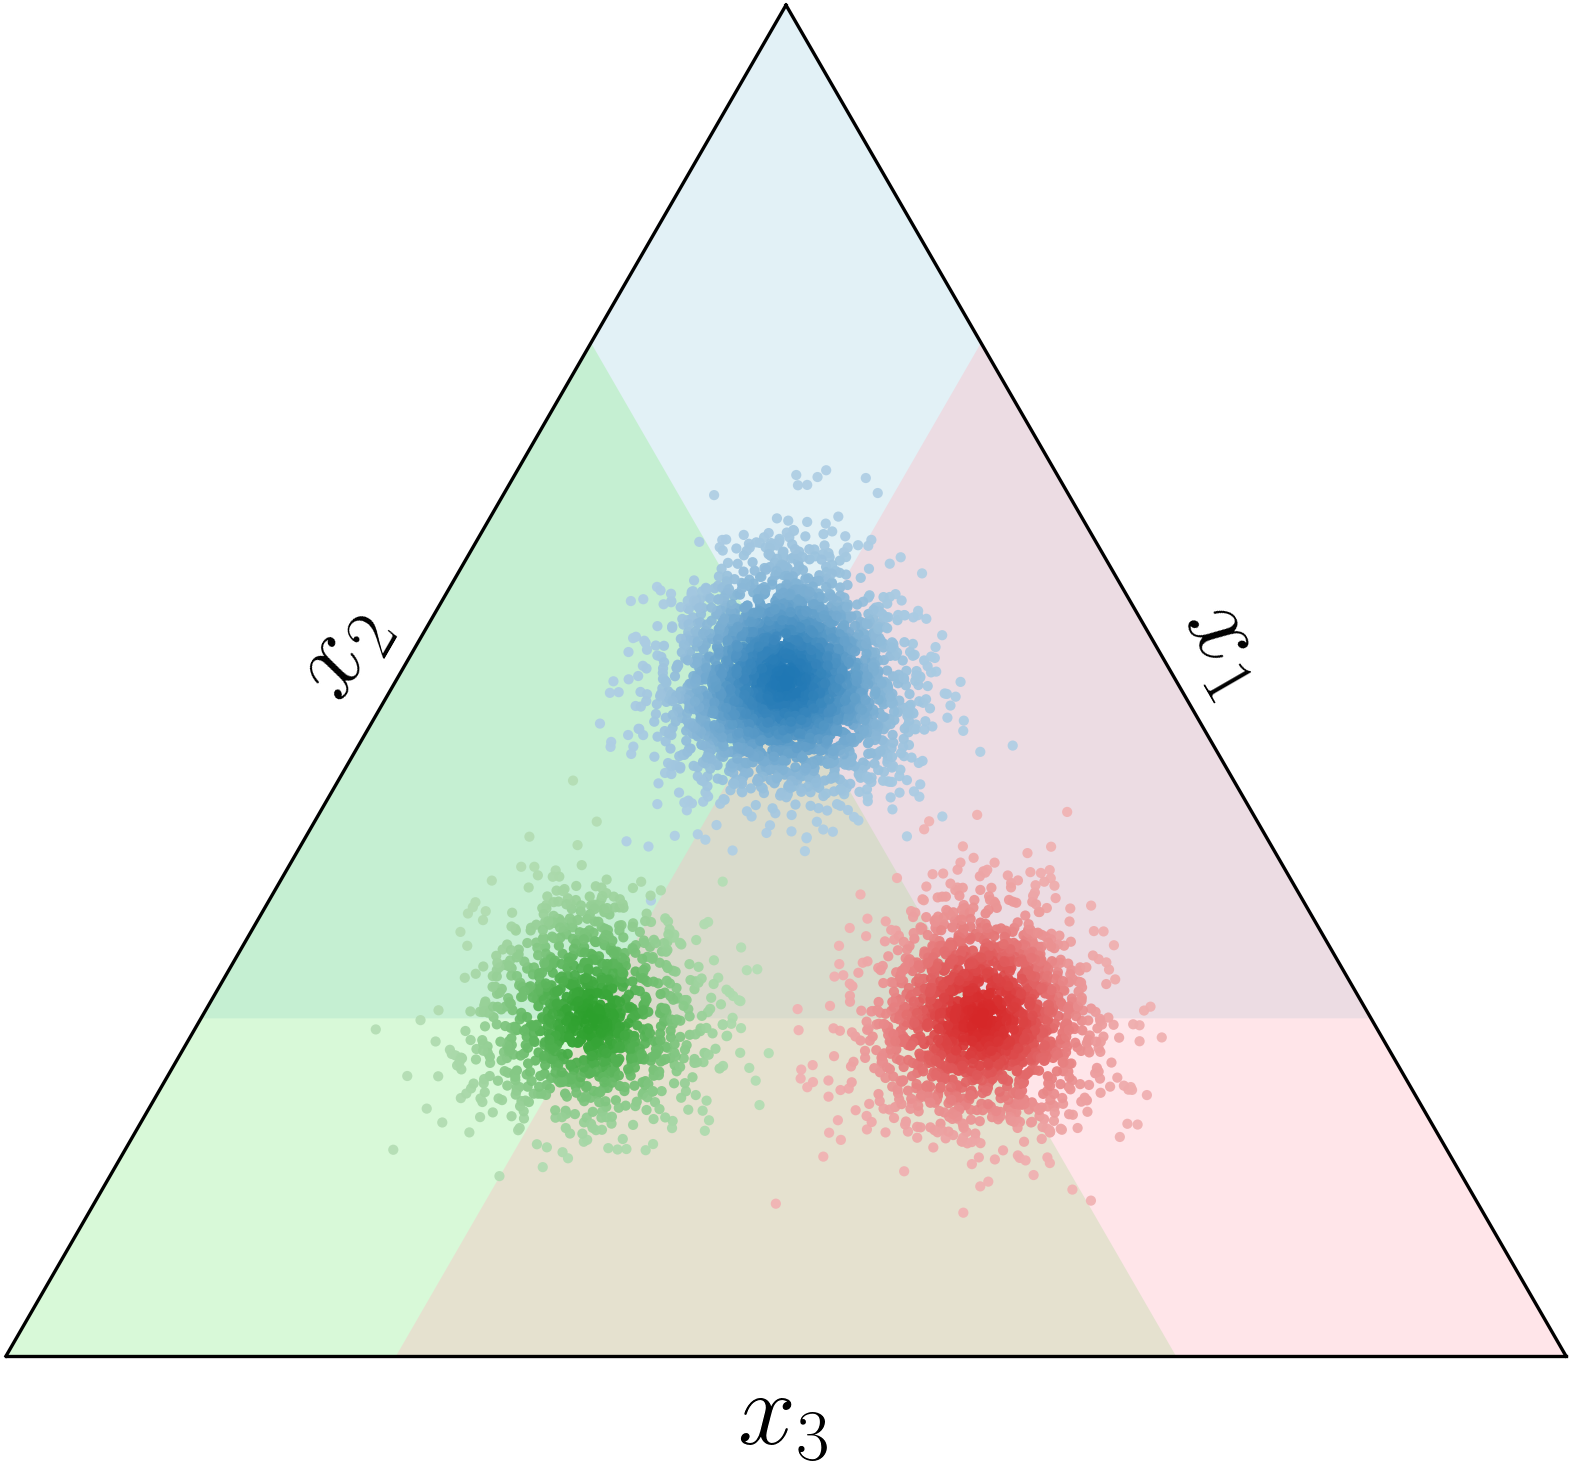
\includegraphics[width=\linewidth]{figs/paper3/lambd_0.25.png}
        \caption*{$\lambda=\tfrac{1}{4}$}
    \end{subfigure}
    \begin{subfigure}{0.3\linewidth}
        \centering
        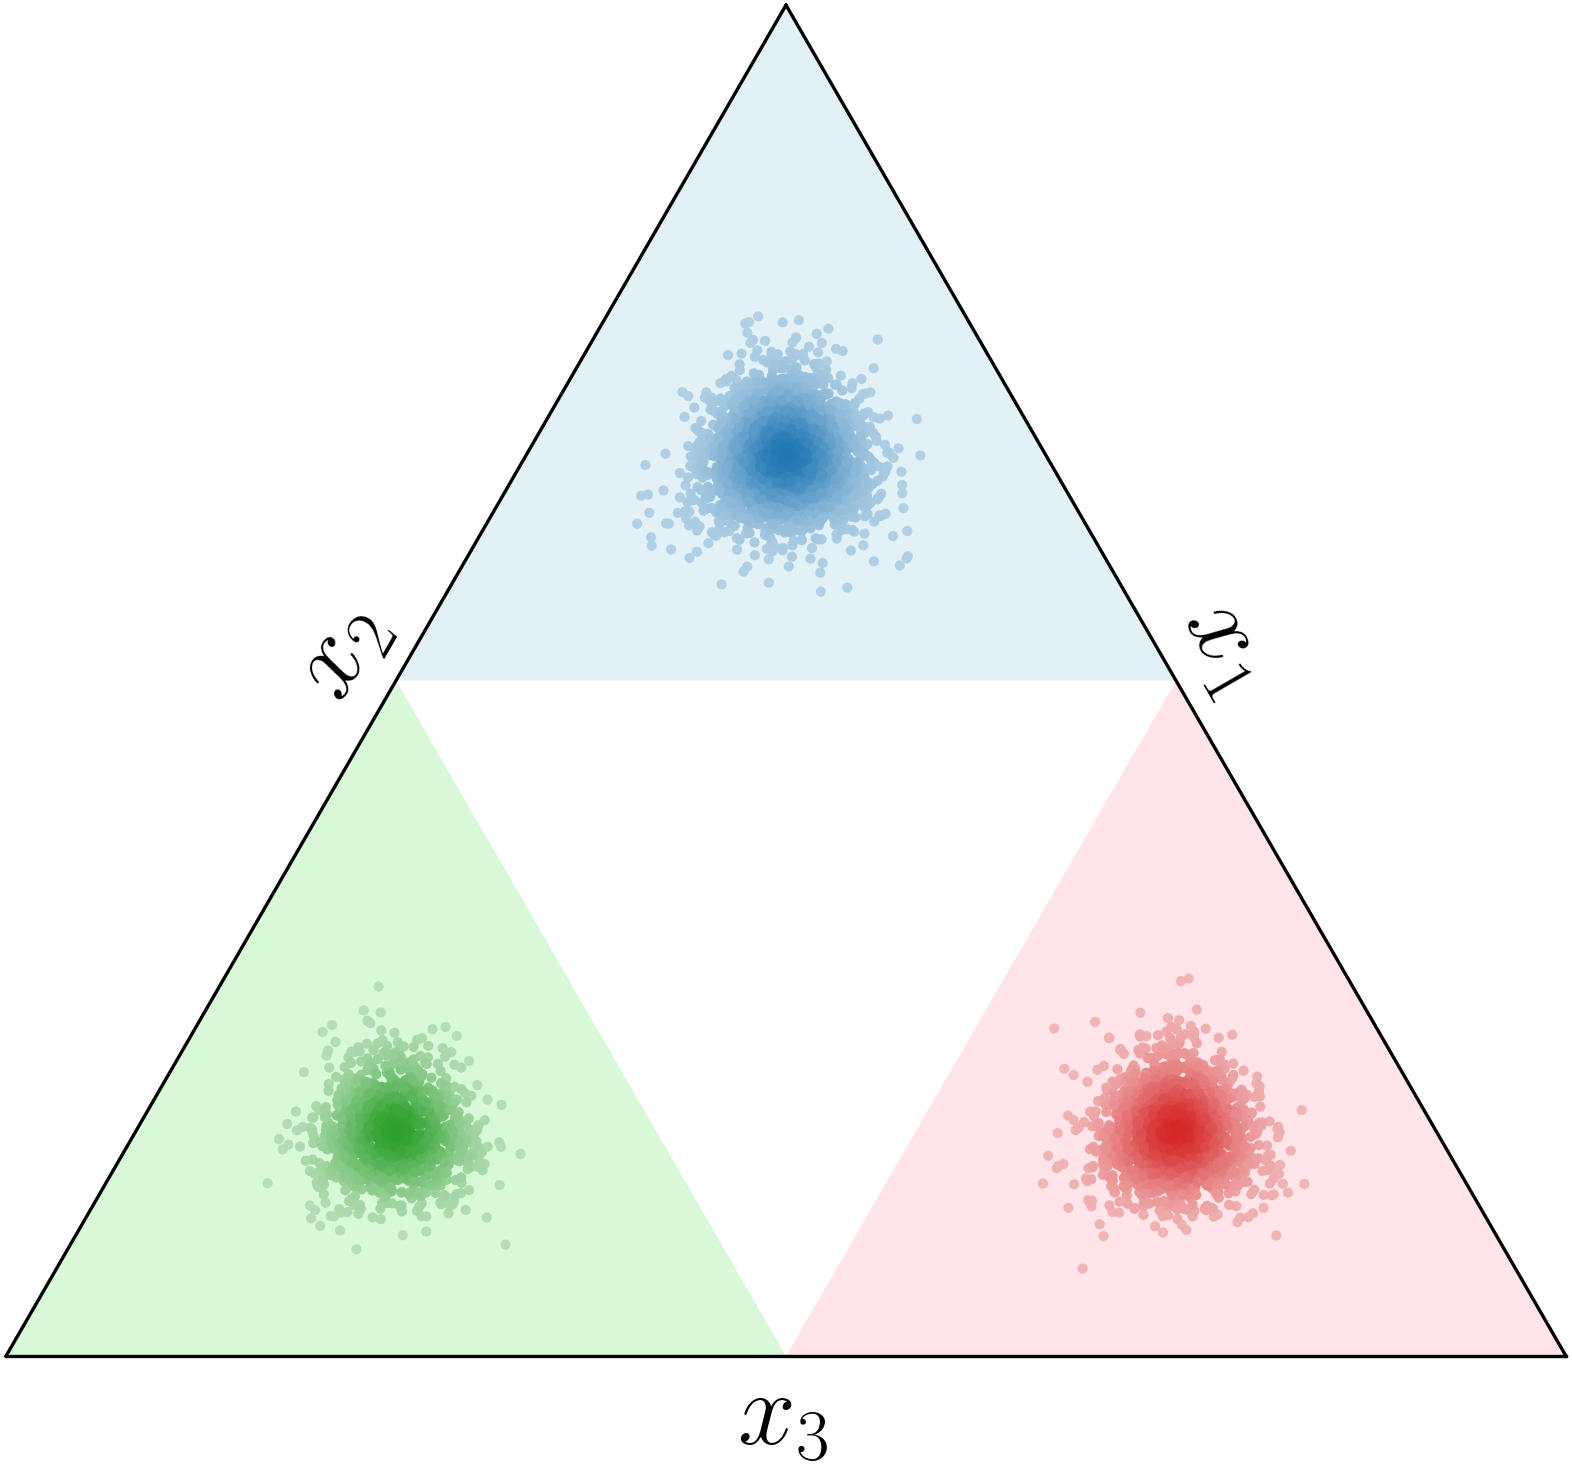
\includegraphics[width=\linewidth]{figs/paper3/lambd_0.5.png}
        \caption*{$\lambda=\tfrac{1}{2}$}
    \end{subfigure}
    \begin{subfigure}{0.3\linewidth}
        \centering
        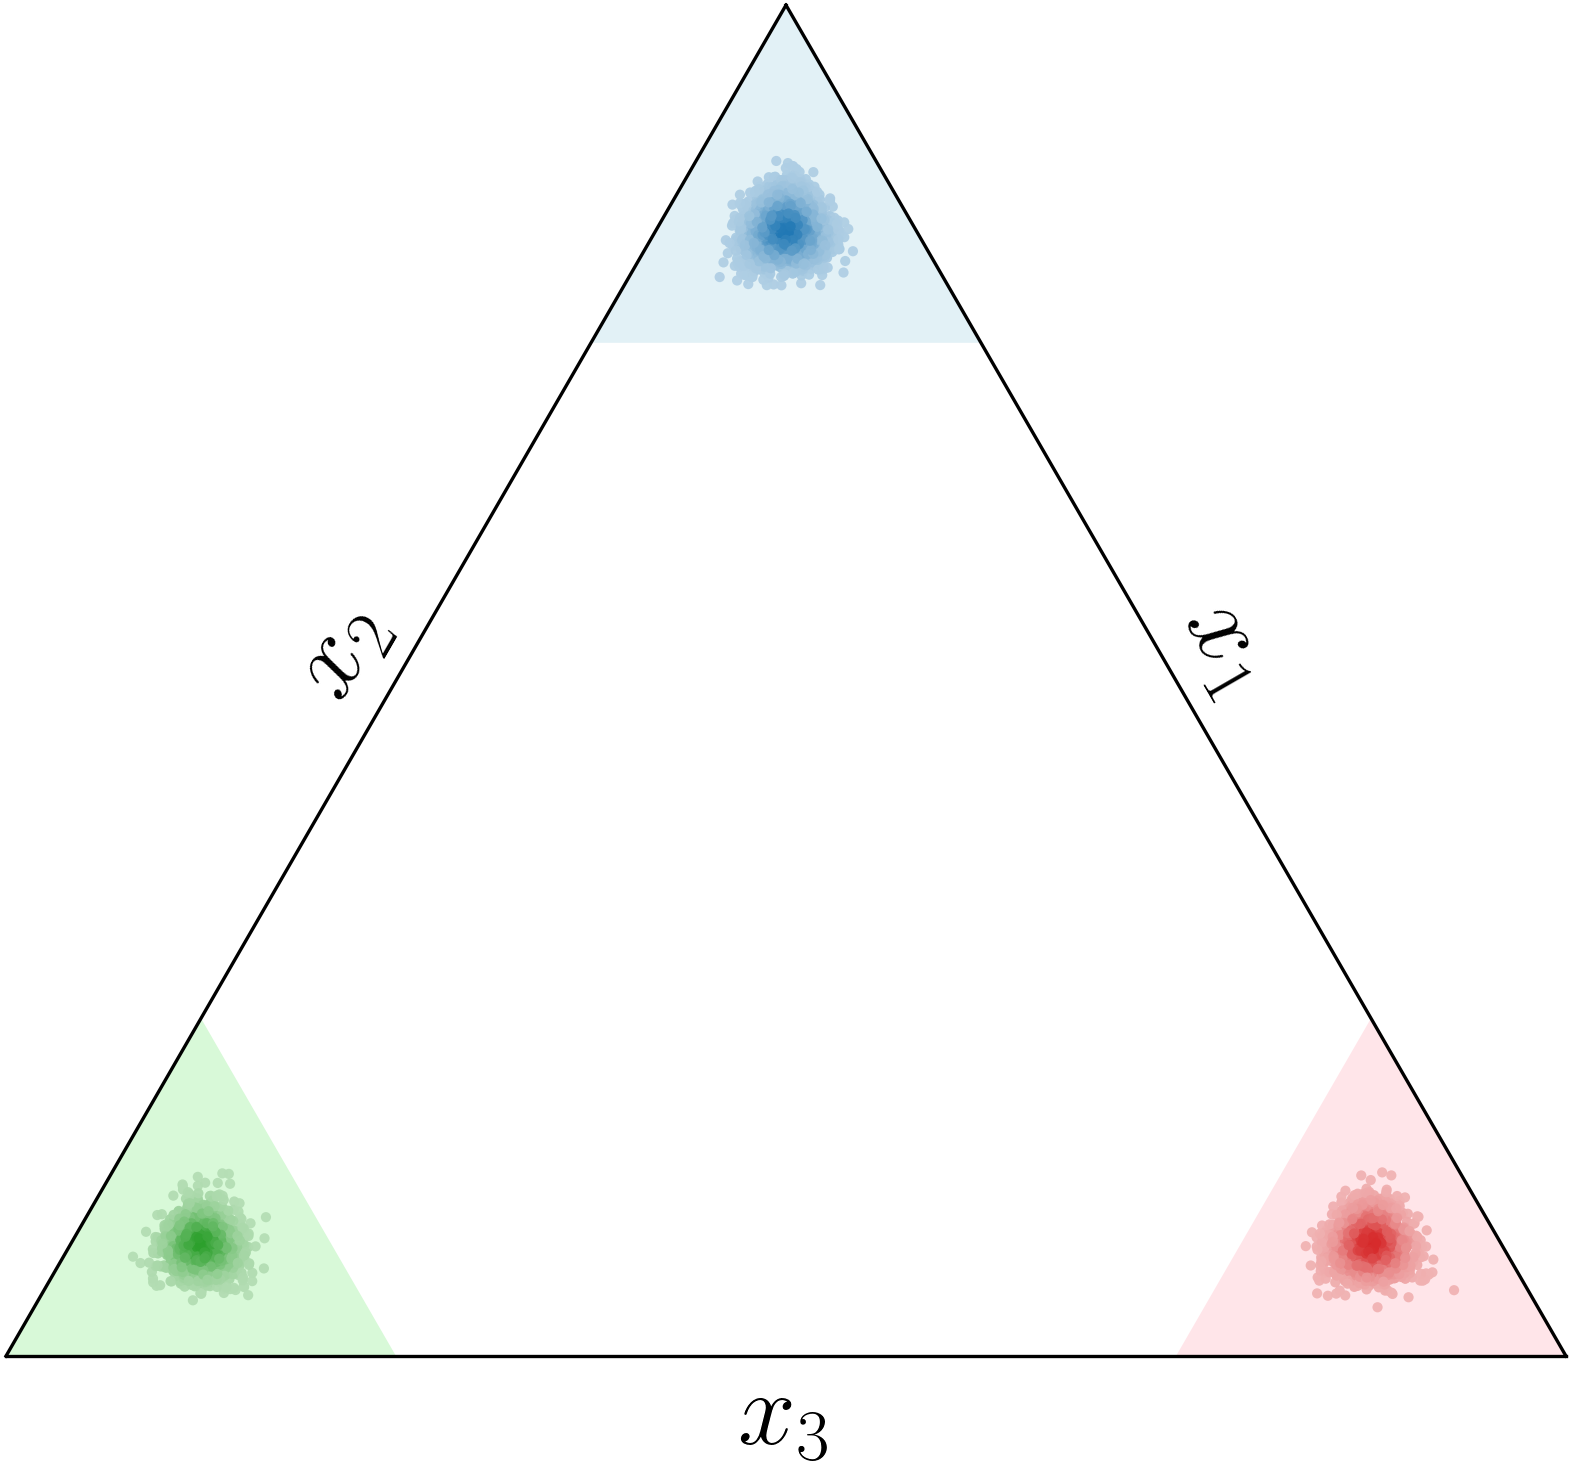
\includegraphics[width=\linewidth]{figs/paper3/lambd_0.75.png}
        \caption*{$\lambda=\tfrac{3}{4}$}
    \end{subfigure}
    \caption{Dirichlet interpolation. The $\lambda$ parameter controls the mixture distribution. For $\lambda \ge \tfrac{1}{2}$ the supports do not overlap and we can recover the categories almost surely. Large $\lambda$ unnecessarily concentrates the mass around the simplex borders we want to avoid.  $\lambda=\tfrac{1}{2}$ illustrates  the $\arg\max$ regions by  the different color blocks.
}
    \label{fig:lambda}
\end{figure}


\paragraph{Latent Gaussian interpolation}
In some cases it is more convenient to place the distribution of the noise process directly on Euclidean latent space. We do this by first interpolating in the simplex space, mapping to Euclidean space with the bijection and adding noise there. For each class $k$, define the interpolated point
\begin{equation}
    \boldsymbol\mu^{(k)} := \lambda\,\boldsymbol e_k + (1-\lambda)\,\tfrac{1}{K}\boldsymbol 1 \in \mathring\Delta^{D},
\qquad \lambda\in(0,1),
\end{equation}
and map it to the latent mean vector $\boldsymbol{m}^{(k)} = \varphi(\boldsymbol\mu^{(k)})$. We then define the latent Gaussian interpolation
\begin{equation}
\boxed{
\boldsymbol z\mid c=k
\sim
\mathcal N\!\bigl( \boldsymbol{m}^{(k)},\,\sigma^2\mathbf I_D\bigr).
}
\label{eq:lik}
\end{equation}

The discrete labels are distributed as $c\sim\mathrm{Cat}(\pi_1,\dots,\pi_K)$, where the class-probability vector $\boldsymbol{\pi}\in\Delta^D$ is unknown.
The distribution in latent space is a Gaussian mixture (see Figure~\ref{fig:likelihood}) centered at $\boldsymbol m^{(k)}$. This can be seen by marginalizing over the classes,
\begin{equation*}
\begin{aligned}
p(\boldsymbol z) = \sum_{k=1}^K p(c=k)\, p(\boldsymbol z\mid c=k) = \sum_{k=1}^K \pi_k\,\mathcal N\!\bigl(\boldsymbol z\mid \boldsymbol m^{(k)},\,\sigma^2\mathbf I_D\bigr).
\end{aligned}
\end{equation*}
\begin{figure}
    \centering
    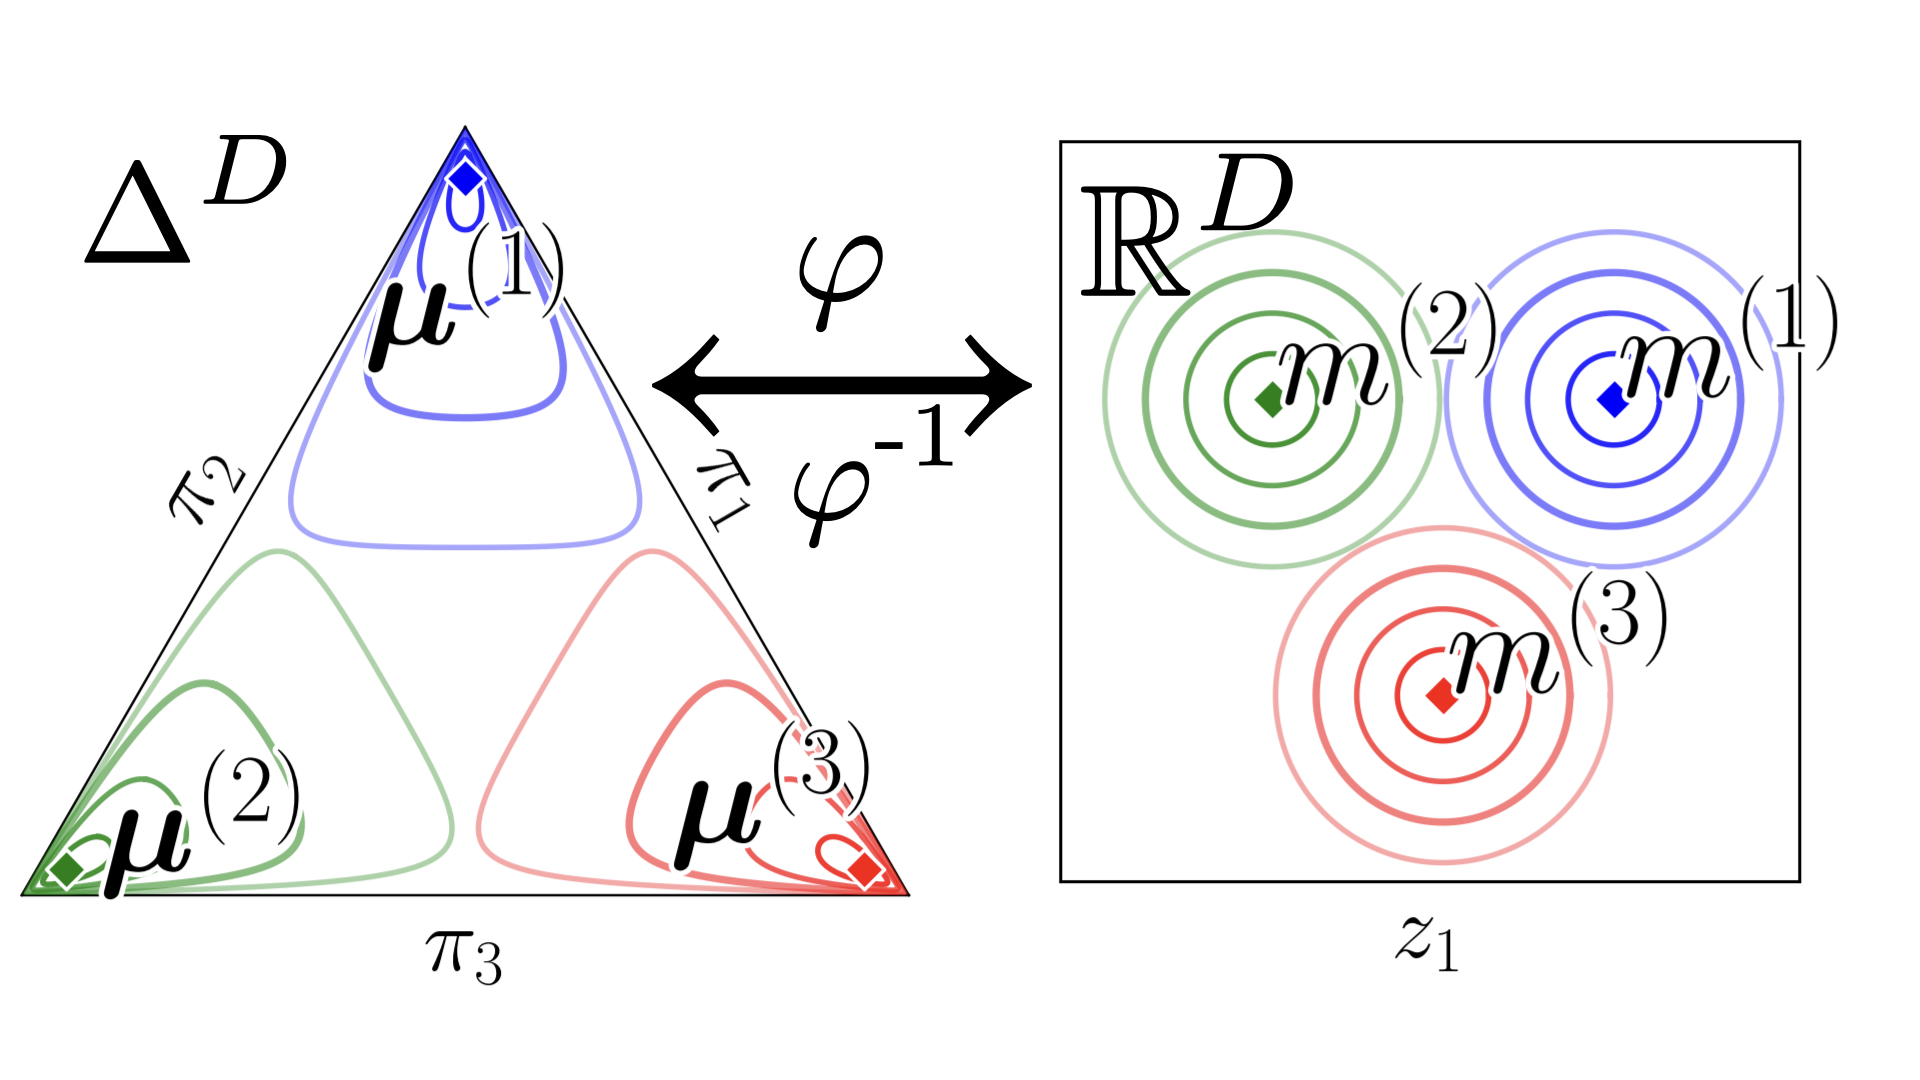
\includegraphics[width=0.8\linewidth]{figs/paper4/lik.001.jpeg}
    \caption{The likelihood of observing classes $1$, $2$, or $3$ is a Gaussian mixture with  modes at $\boldsymbol m^{(k)}=\varphi(\boldsymbol\mu^{(k)})$ in Euclidean space (right), which induces a pushforward likelihood on the simplex (left). The figure shows the likelihood for class probabilities $\boldsymbol{\pi} = (1/3,1/3,1/3)$.}
    \label{fig:likelihood}
\end{figure}

The design choice is the value $\sigma^2$. This parameter controls the overlap between the components, and we can relate this overlap to the probability of the stochastic interpolation being in the incorrect $\arg\max$ region. The key insight is the isometry: distances in the latent space equal distances in the open simplex
\[
\delta := d_A\!\bigl(\boldsymbol\mu^{(k)},\boldsymbol\mu^{(\ell)}\bigr) = \|\boldsymbol m^{(k)}-\boldsymbol m^{(\ell)}\|_2,\qquad k\neq \ell,
\]
and the probability of misclassification is the probability of being closer in Euclidean distance to $\boldsymbol m^{(j)}$ than to the correct mode $\boldsymbol m^{(k)}$.
Proposition~\ref{prop:sigma_bound} gives a sufficient condition on $\sigma$ to make the probability of leaving the correct region (misclassification) smaller than a prescribed tolerance $\varepsilon$.


\begin{proposition}[Proposition 1, Paper IV]\label{prop:sigma_bound}
Let $K\ge 2$.  Define, for each class $k\in\{1,\dots,K\}$,
\[
 \boldsymbol m^{(k)} := \varphi\!\bigl(\boldsymbol\mu^{(k)}\bigr)\in\mathbb R^{D}, \quad \delta := \|\boldsymbol m^{(k)}-\boldsymbol m^{(\ell)}\|_2, \quad k\neq \ell,
\]
where $\delta$ is the Aitchison distance between the class centers on the simplex by the ILR isometry.
Let $\mathcal V_k:=\{\boldsymbol z\in\mathbb R^{D}:\|\boldsymbol z-\boldsymbol m^{(k)}\|_2\le \|\boldsymbol z-\boldsymbol m^{(\ell)}\|_2\ \forall \ell\}$.
For any $\varepsilon\in(0,1)$, if
\begin{equation}\label{eq:sigma_bound}
\sigma \;\le\; \frac{\delta}{2\; z_{1-\varepsilon/D}},
\qquad z_{q}:=\Phi^{-1}(q),
\end{equation}
where $\Phi$ is the standard normal CDF,
then for every $\boldsymbol{x}\in \mathring\Delta^D$ and every $k\in\{1,..,K\}$, the probability of miss-classification is bounded by $\varepsilon$,
\[
\mathbb P\!\big(\boldsymbol Z\notin \mathcal V_k \,\big|\, C=k,\boldsymbol{x}\big)\;\le\;\varepsilon,
\]
where $C$ denotes the class label and $\boldsymbol Z\sim\mathcal N(\boldsymbol m^{(k)},\sigma^2\mathbf I_D)$.
\end{proposition}





\section{Case Study III: Categorical Flow Matching}
This case study combines Flow Matching introduced in Section~\ref{sec:discrete_data} with the simplex-to-Euclidean bijections and the stochastic interpolations developed in this chapter. The proposed method is Simplex-to-Euclidean Flow Matching, where the generative model is trained on Euclidean coordinates but produces samples on the simplex.

Unlike Statistical Flow Matching \citep{Cheng2024, Davis2024}, which uses the Fisher geometry of the simplex and performs Riemannian flow matching on the sphere, our method does not learn the flow on a curved manifold. Instead, we map the problem to $\mathbb{R}^D$, where Euclidean conditional flow matching is applied. This removes the need for Riemannian operations such as the exponential and logarithm maps during training and sampling.

\paragraph{Simplex-to-Euclidean Flow Matching (FM-$\mathring\Delta$)}
Algorithm~\ref{alg:train} details the training procedure of our method. If the data is in the interior of the simplex then the bijection is enough, but if the data is discrete on the boundary, we first use the stochastic interpolation to move the data to the interior and then apply the bijection $\varphi$ and train the Euclidean flow. During sampling the $\arg\max$ converts the continuous process to discrete predictions.
Sampling is done with the procedure specified in Algorithm~\ref{alg:sample_sfm} with an additional $\arg\max$ operator if the generated data is discrete. Any of the simplex-to-Euclidean bijections can be used within the method, and the accuracy is affected by this choice. These include additive logratio, multiplicative log ratio, stick-breaking, and isometric logratio.
Note that using conditional flow matching is a design choice, the procedure is valid for any continuous Euclidean generative model, for example diffusion models \citep{song2021score, Karras2024}.

\begin{algorithm}
\caption{Training of Simplex-to-Euclidean Flow Matching.}
\label{alg:train}
\begin{algorithmic}[1]
\Require Data $\boldsymbol{c}\!\in\!\Delta^{D}$, weight $\lambda\!\in\!(0,1)$, 
Dirichlet $\alpha>0$, bijection $\varphi$, base $p_0$ (e.g. $\mathcal{N}(\boldsymbol{0},\boldsymbol{I})$), 
coupling $\pi$ (indep. or minibatch OT), isDiscrete
\For{each mini-batch}
  \For{each $\boldsymbol{c}$ in batch}
    \If{isDiscrete}
      \State Sample $\boldsymbol{\varepsilon}\!\sim\!\mathrm{Dir}(\alpha,..,\alpha)$
      \State ${\boldsymbol{x}} \gets \lambda \boldsymbol{c}+(1-\lambda)\boldsymbol{\varepsilon}$
    \Else
      \State ${\boldsymbol{x}} \gets \boldsymbol{c}$
    \EndIf
  \EndFor
  \State $\boldsymbol{z}_1 \gets \varphi({\boldsymbol{x}})$ \Comment{Map to Euclidean space.}
  \State Sample $\boldsymbol{z}_0 \sim p_0$; pair $(\boldsymbol{z}_0,\boldsymbol{z}_1)$ via $\pi$
  \State Sample $t\sim \mathrm{Unif}(0,1)$
  \State $\boldsymbol{z}_t\!\gets\!(1-t)\boldsymbol{z}_0+t \boldsymbol{z}_1$, \;
         $\boldsymbol{u}_t\!\gets\!\boldsymbol{z}_1-\boldsymbol{z}_0$
  \State Update $\theta$ by 
  $\min \|\boldsymbol{v}_\theta(\boldsymbol{z}_t,t)-\boldsymbol{u}_t\|^2$ \; (Equation~\ref{eq:cfm_loss})
\EndFor
\end{algorithmic}
\end{algorithm}

Proposition~\ref{prop:cat_prob_tv} justifies the correctness of FM-$\mathring\Delta$ for categorical data, it states that if the learned flow model matches the distribution of the interpolated data with the stochastic interpolation, then the true unknown probabilities are recovered by the model's $\arg\max$ estimations. 


\begin{proposition}[Proposition 1, Paper III] \label{prop:cat_prob_tv}
\textbf{Categorical probabilities bound:}
Let $\lambda \ge \tfrac{1}{2}$ so that the Dirichlet-interpolated mixture
$q_\lambda(\boldsymbol{x})=\sum_{k=1}^{K} \pi_k\, q_\lambda(\boldsymbol{x}\mid \boldsymbol{e}_k)$ 
has a.s. disjoint component supports contained in the strict $\arg\max$ regions
$\mathcal{R}_k := \{ \boldsymbol{x}\in \mathring \Delta^{D} : x_k > x_j\ \forall j\neq k\}.$
For any density $\tilde q$ on $\mathring \Delta^D$ define the induced (generated) categorical probabilities
$\hat \pi_k := \int_{\mathcal{R}_k} \tilde q(\boldsymbol{x})\,d\boldsymbol{x}.$
Then the total variation between the true and generated categorical laws is bounded by the $L^1$ distance between the distributions:
\begin{equation*}
\mathrm{TV}(\boldsymbol{\pi},\hat{ \boldsymbol{\pi}})= \tfrac{1}{2}\sum_{k=1}^{K} | \hat \pi_k - \pi_k |
\;\le\; \tfrac{1}{2}\,\|\tilde q - q_\lambda\|_{1}.
    \end{equation*}
In particular, $\|\tilde q - q_\lambda\|_{1}\to 0$ implies $\hat{\boldsymbol{\pi}} \to \boldsymbol{\pi}$ in total variation, and the $\arg\max$ discretization of $\tilde q$ recovers exactly the true categorical distribution.
\end{proposition}






\subsection*{Empirical evaluation}
We highlight two experiments from Paper~III that illustrate the two parts of the construction. The first considers a density supported on the open simplex, where the role of the bijection and geometry can be seen directly. The second is a language-generation task on discrete data, where the full pipeline including stochastic interpolation is needed. The main comparison methods are LinearFM which uses Euclidean geometry on the simplex itself and Statistical Flow Matching (SFM) \citep{Cheng2024, Davis2024}.

\paragraph{Density on the open simplex}
This experiment considers checkerboard data projected to the open simplex. The data is continuous in $\mathring\Delta^2$, so no interpolation is needed in this comparison. The experiment studies the effect of the geometric representation (simplex, simplex-to-sphere, or simplex-to-Euclidean) and two different choices of bijection (SB or ILR). Figure~\ref{fig:checkboard} shows that our method produces samples that align more closely with the target density than both LinearFM and SFM. In particular, the Euclidean baseline on the simplex and the Fisher-sphere construction produce many more invalid samples near the corners, whereas the simplex-to-Euclidean approach better preserves the structure of the target. Both the isometric logratio and stick-breaking bijections work well, with stick-breaking performing slightly better in this example.
\begin{figure}
    \centering
    \begin{subfigure}[b]{0.4\linewidth}
        \centering
        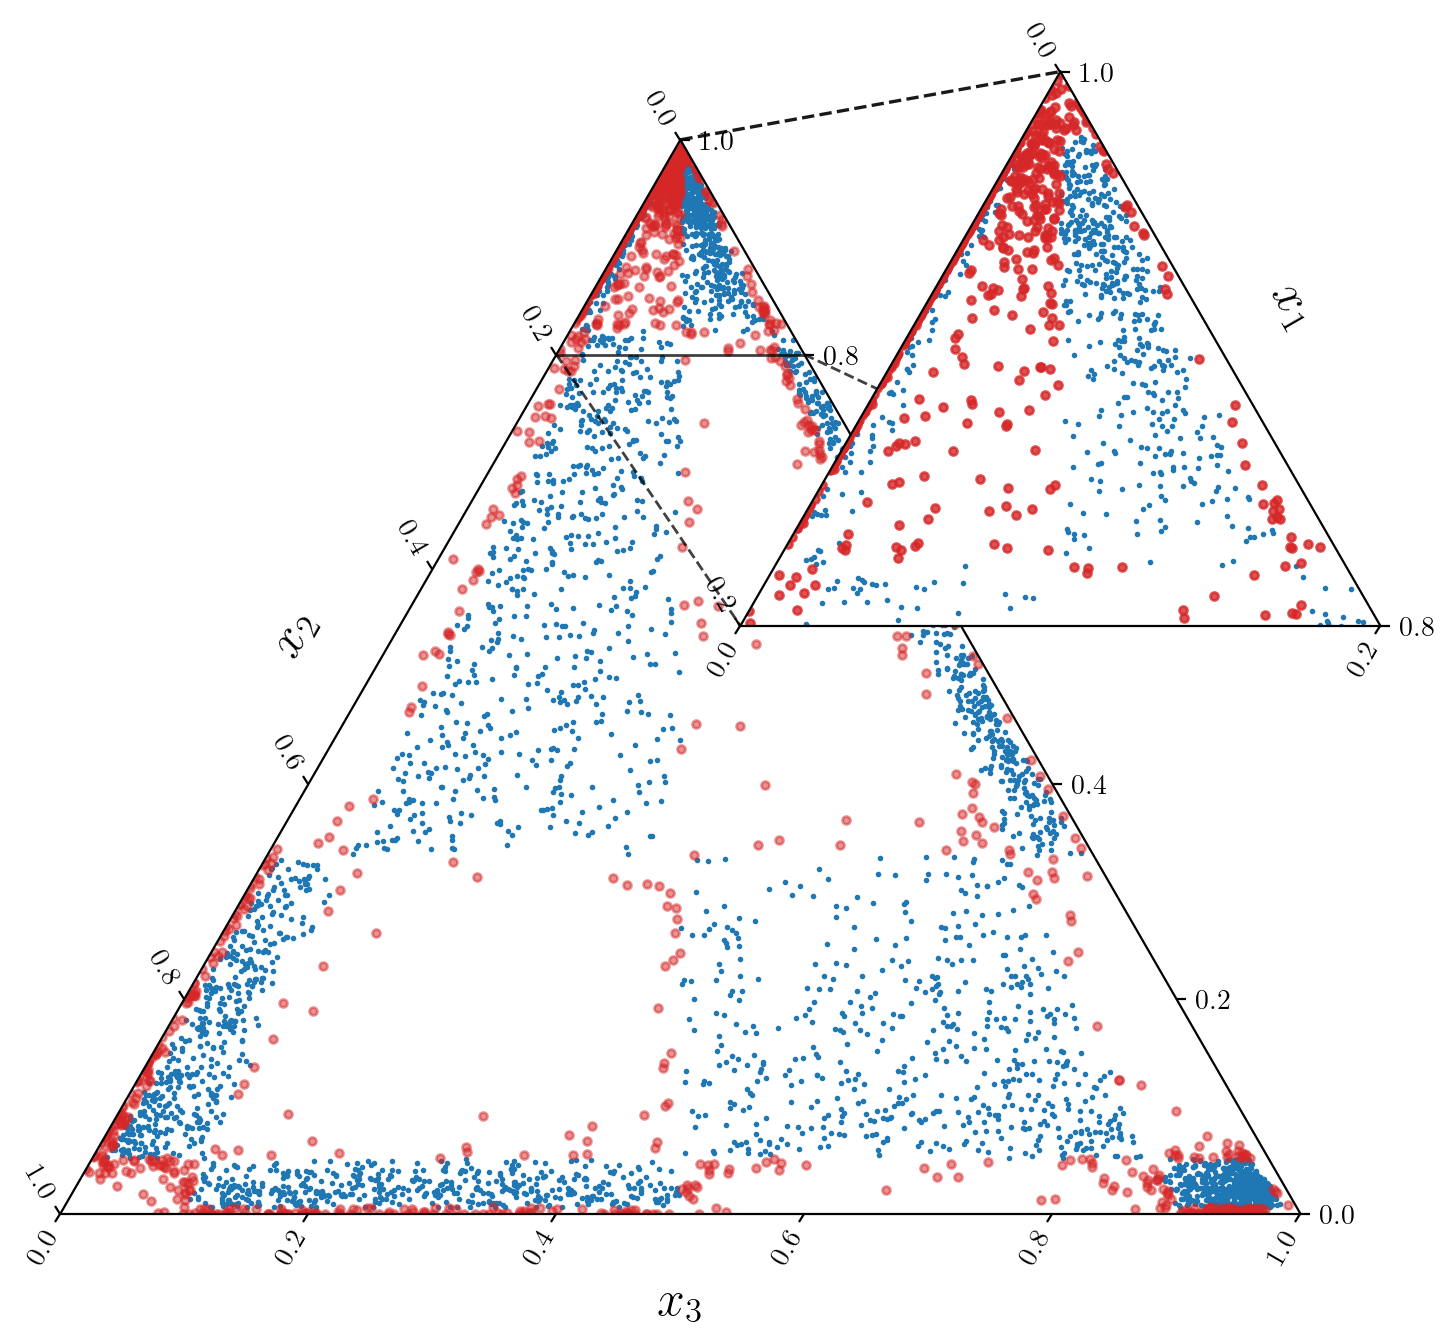
\includegraphics[width=\linewidth]{figs/paper3/checkerboard/linear.png}
        \caption{\footnotesize LinearFM\\ $25.9\%$}
    \end{subfigure}
    \begin{subfigure}[b]{0.4\linewidth}
        \centering
        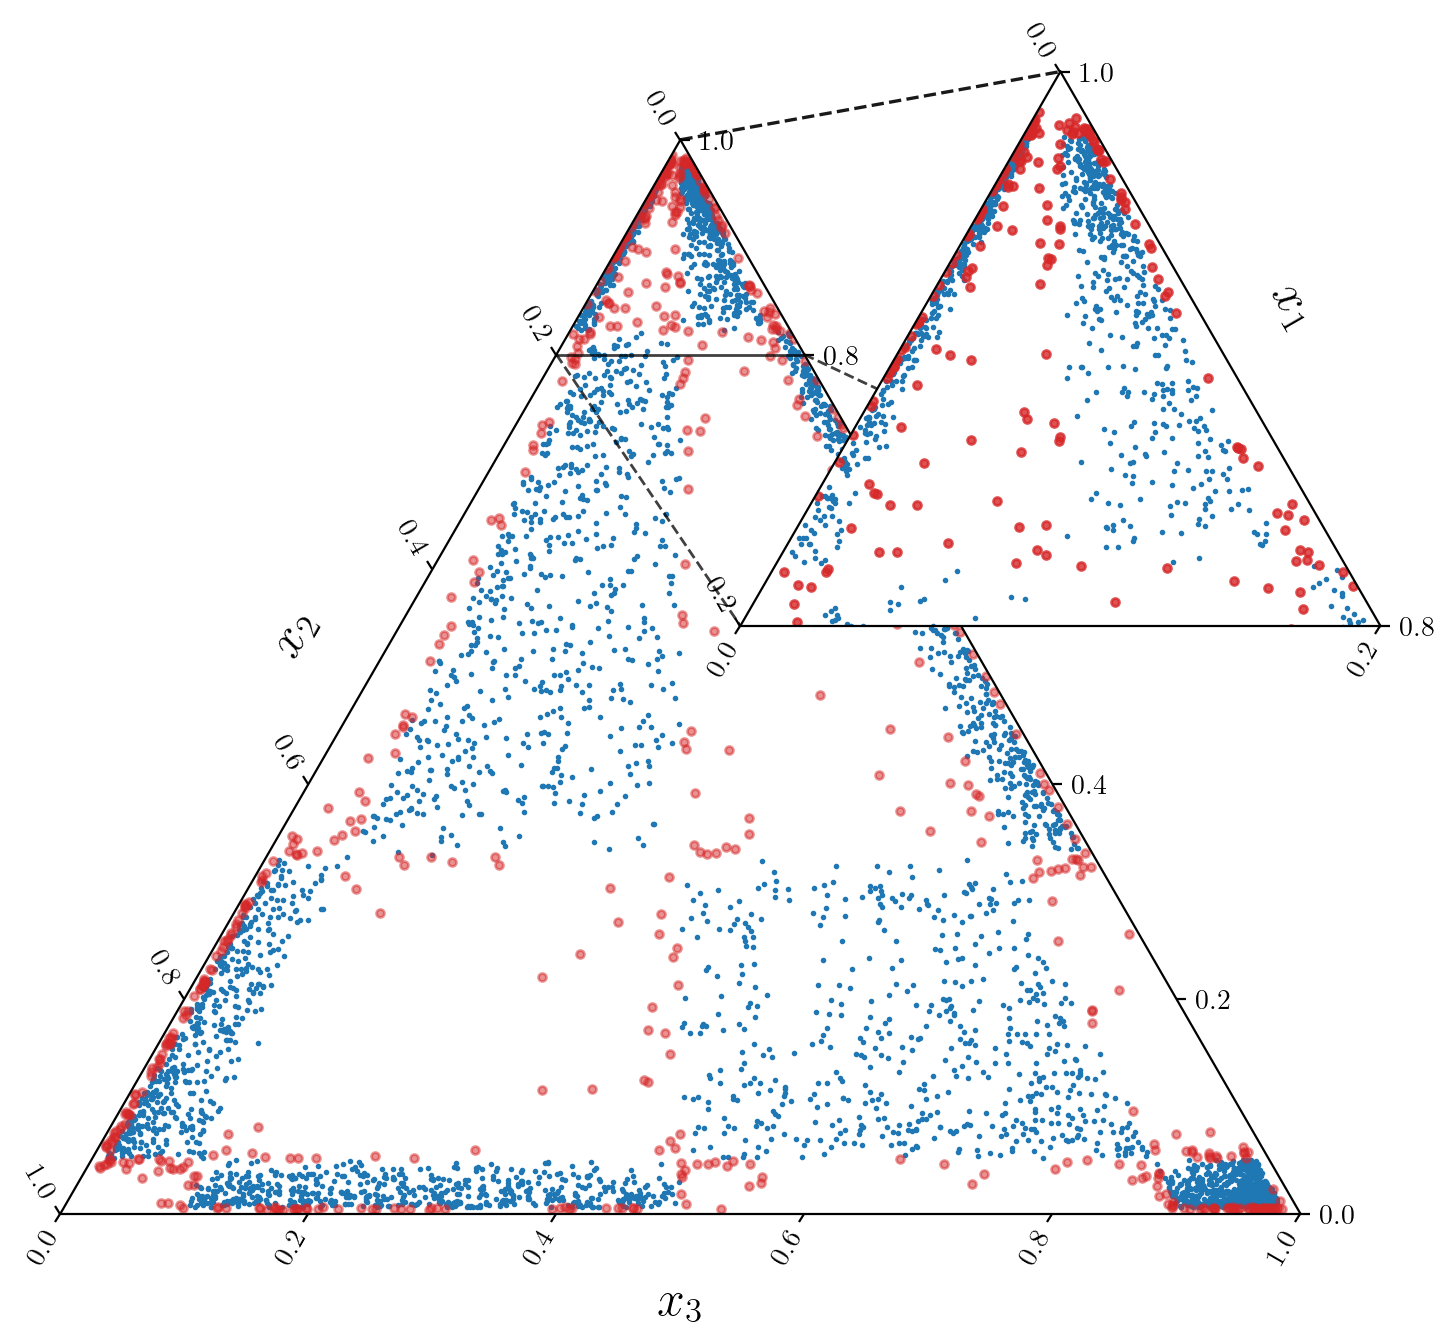
\includegraphics[width=\linewidth]{figs/paper3/checkerboard/sphere.png}
        \caption{\footnotesize SFM\\ $12.9\%$}
    \end{subfigure}
    \begin{subfigure}[b]{0.4\linewidth}
        \centering
        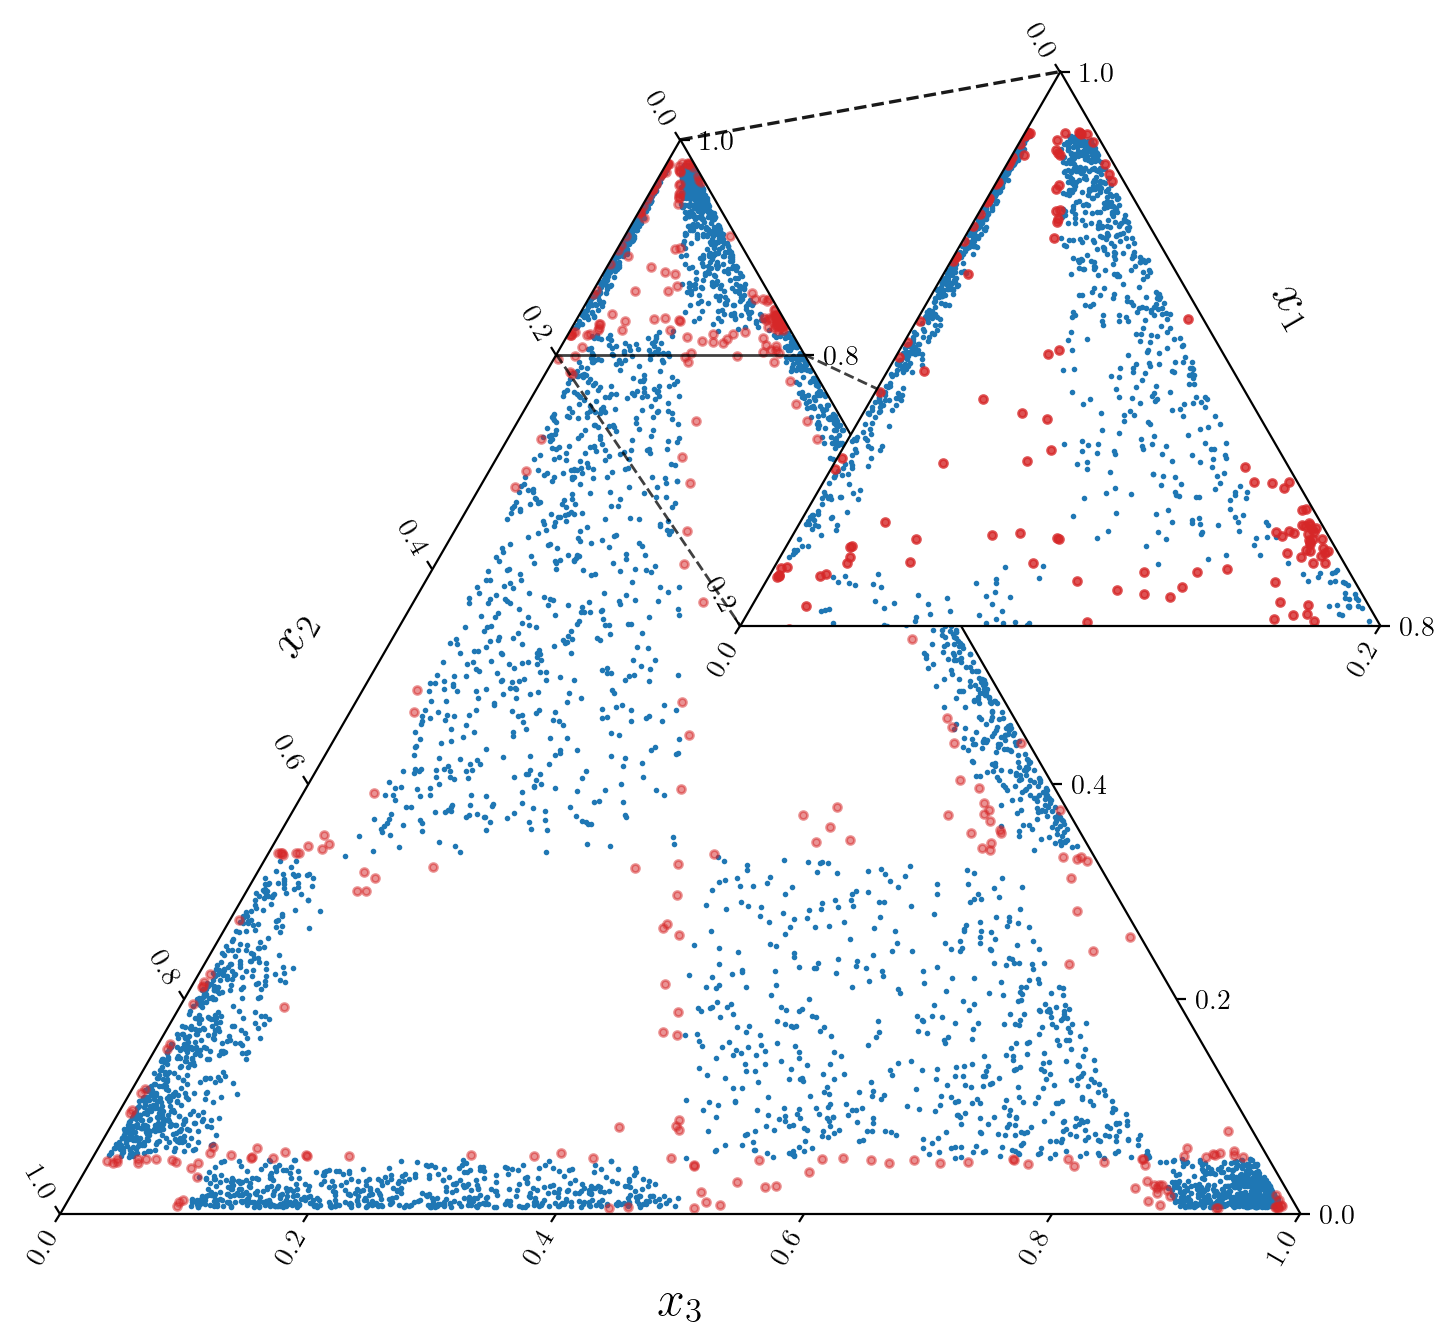
\includegraphics[width=\linewidth]{figs/paper3/checkerboard/ilr.png}
        \caption{ \footnotesize FM-$\mathring\Delta$(ILR)\\ $6.8 \%$}
    \end{subfigure}
    \begin{subfigure}[b]{0.4\linewidth}
        \centering
        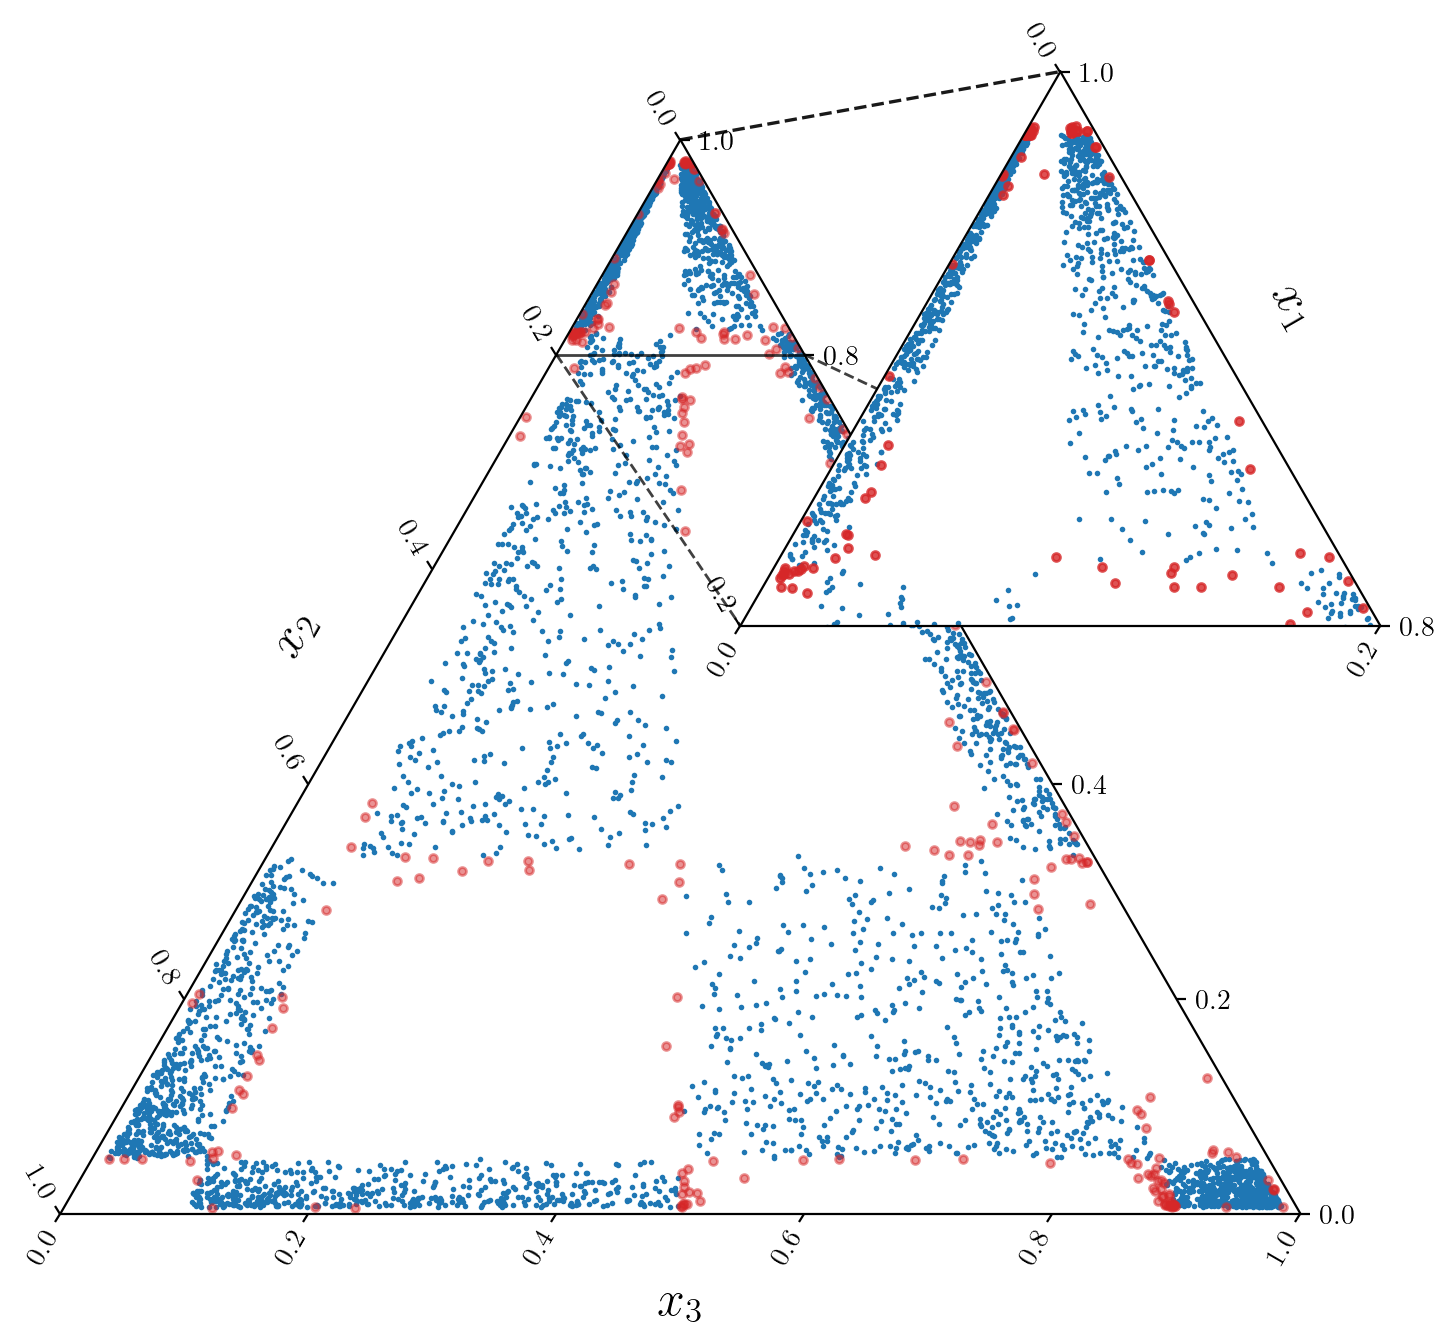
\includegraphics[width=\linewidth]{figs/paper3/checkerboard/sb.png}
        \caption{\footnotesize FM-$\mathring\Delta$(SB)\\ $5.4 \%$}
    \end{subfigure}
    \caption{Samples from Checkerboard on the simplex. Red points indicate samples not aligned with the true density ($\%$ indicated in caption). The zoomed area shows the top region $x_1\geq \tfrac{4}{5}$, emphasizing the differences. }
    \label{fig:checkboard}
\end{figure}

\paragraph{Language generation}
We consider the Text8 dataset \citep{Mahoney2011}, which consists of $K=27$ categories: $26$ letters and the space character, split into random chunks of size $256$. This task illustrates the full discrete-data setting, and we rely on Dirichlet interpolation to move the data to the open simplex, followed by a Euclidean flow model in latent coordinates. We use an auto-regressive model to evaluate the NLL and compute the entropy \citep{Wang2021}; the NLL should be low and the entropy over generated data should be close to the entropy of the test data.
Table~\ref{tab:text8} shows the NLL, entropy, and difference in entropy. It shows that our method is the most competitive among the continuous approaches and improves over LinearFM and SFM. However, the best overall result is obtained by the discrete-state diffusion model SEDD \citep{Lou2024}. SEDD is a discrete diffusion model that operates directly in the discrete space. At the time of submission of our method there was still a gap between latent continuous models and discrete diffusion models, which has been closing recently \citep{lee2026flow}. The outcome is that Simplex-to-Euclidean Flow Matching is a strong continuous baseline, even if it does not fully close the gap to the best discrete-state models.





\begin{table}[t]
\centering
\caption{Text8: NLL and Entropy on the GPT-J-6B model. The baseline results are taken from the respective papers.}
\label{tab:text8}
\begin{tabular}{cllccc}
\cline{2-5}
 & \textbf{Model} & \textbf{NLL $\downarrow$} & \textbf{Entropy} & \textbf{Diff} \\
\cline{2-5}
\multirow{6}{*}{\rotatebox[origin=c]{90}{{\textbf{Discrete}}}}
 & MDLM            & 6.76 & 7.55 & +0.07 \\
 & DFM             & 6.78 & 7.58 & +0.10 \\
 & D3PM            & 6.93 & 7.38 & -0.10 \\
 & SEDD   & \textbf{6.49} & 7.17 & -0.31 \\
 & MultiFlow       & 6.73 & 7.39 & -0.09 \\
\cline{2-5}
\multirow{8}{*}{\rotatebox[origin=c]{90}{{\textbf{Continuous}}}}
 & LinearFM          & 7.35 & 7.62 & +0.14 \\ 
 & $\alpha$-Flow($\alpha{=}{-}0.5)$  & 7.14 & 7.37 & -0.11 \\
 & $\alpha$-Flow($\alpha{=}0.5$)     & 7.00 & 7.42 & -0.06 \\
 & $\alpha$-Flow($\alpha{=}1$)       & 7.09 & 7.51 & \textbf{+0.03} \\
 & SFM             & 6.85 & 7.38 & -0.10 \\ 
 \cdashline{2-5}
 & FM-$\mathring\Delta$(ILR)         & 6.81 & 7.39 & -0.09 \\
 & FM-$\mathring\Delta$(ILR)w{/}OT   & 6.89 & 7.38 & -0.10 \\
\cline{2-5}
 & Data & 4.10 & 7.48 & 0 \\
\cline{2-5}
\end{tabular}
\end{table}



\section{Case Study IV: Gaussian Process Classification}
This case study uses the isometric logratio and the latent Gaussian interpolation to build a multiclass Gaussian process classifier that is conjugate in latent space. Similar to Case Study III, the idea is to map the simplex-valued problem to Euclidean coordinates and then apply a standard continuous model there, in this case the model is Gaussian process regression. We present the method and show with empirical studies that it is accurate and well-calibrated. 


\paragraph{Isometric Logratio Gaussian Process }
Denote the training data as $\{(\boldsymbol r_i,c_i)\}_{i=1}^N$, where $\boldsymbol r_i$ denotes the regressor and $c_i\in\{1,\dots,K\}$ the class label. The construction uses the ingredients introduced earlier in the chapter. Each label $c_i=k$ is moved to the interior of the simplex with the interpolation
\begin{align*}
\boldsymbol\mu^{(k)}&=\lambda\,\boldsymbol e_k + (1-\lambda)\tfrac{1}{K}\boldsymbol 1, 
\end{align*}
and then mapped to Euclidean space with the ILR bijection (Equation~\ref{eq:ilr}) $\varphi$ giving the latent $\boldsymbol m^{(k)}=\varphi(\boldsymbol\mu^{(k)})$. The latent Gaussian likelihood (Equation~\ref{eq:lik}) together with the misclassification probability bound (Proposition~\ref{prop:sigma_bound}), turns classification into GP regression in $\mathbb{R}^D$. The model is
\begin{equation}
\boxed{
\mathbf f(\cdot) \sim \mathcal{GP}(\mathbf 0, K_{\theta}),
\qquad
\boldsymbol z_i\mid \mathbf f(\boldsymbol r_i) \sim \mathcal N\!\bigl(\mathbf f(\boldsymbol r_i),\,\sigma^2\mathbf I_D\bigr).
}
\end{equation}
Since the prior and the likelihood are Gaussian, the model is conjugate in $\mathbb{R}^D$ and posterior inference is exact in $\mathbb{R}^D$. The model uses $D$ latent processes because of the dimensionality of the space. Compared to Dirichlet-based GP classification (Section~\ref{sec:discrete_data}) it requires one less latent process and removes the need for a distributional approximation in the model construction.

For a new regressor $\boldsymbol{r}_*$, class-probability predictions are obtained from the expected value after mapping back to the simplex with $\varphi^{-1}$. Predictions are estimated with Monte Carlo
\begin{equation}
\begin{aligned}
\mathbb E[\boldsymbol\pi_*\mid \boldsymbol{r}_*,\mathcal D] &\approx
\frac{1}{S}\sum_{s=1}^S \varphi^{-1}\!\bigl(\mathbf f_*^{(s)}\bigr) \\
\mathbf f_*^{(s)}&\sim\mathcal N(\boldsymbol\mu_*,\boldsymbol\Sigma_*).
\end{aligned}
\label{eq:gpilr_pred}
\end{equation}
The method's cubic complexity in the size of the training data limits its scalability. For larger data sizes, Paper~IV studies two inducing-point sparse variants. \emph{Uncollapsed-ILR} is a sparse variational classifier that parametrizes the probabilities as $\boldsymbol{\pi} = \varphi^{-1}(\boldsymbol{z})$; the objective factorizes over observations, which allows for mini-batch optimization \citep{Hensman2015}. \emph{Collapsed-ILR} instead keeps the Gaussian process regression in latent space, which is specified with the Collapsed GP regression approximation (see Equation~\ref{eq:lower_bound_collapsed}). The first variant models the probabilities directly while the second approximates the latent GP regression.

\subsection*{Empirical evaluation}
We highlight two experimental evaluations from Paper~IV. The objective of the experiments is to benchmark our work in terms of accuracy and calibration with respect to the existing literature. 
The first studies exact latent inference on small UCI classification tasks, where the full GP posterior can be computed exactly. The second studies larger UCI classification tasks for which we use inducing-point methods for inference. The most important related comparison method is Dirichlet-based Gaussian process (GPD). We additionally include comparisons against models that achieve posterior conjugacy through data augmentation; these are Logistic softmax (LSM) \citep{Galy2020} and Bijective softmax (BSM) \citep{galyfajou2022latent}. We denote by E-ILR our model with exact latent inference, by C-ILR the sparse Collapsed version, and by U-ILR the sparse Uncollapsed version of our method. In all experiments we select the learning rate, data normalization, $\alpha_\varepsilon$ and $\lambda$ using a validation set, and the kernel parameters are optimized with the marginal log likelihood or its lower bound using the training set. We report classification error, negative log-likelihood (NLL), and expected calibration error (ECE).

\paragraph{Exact UCI regression}
We first evaluate the exact ILR model on three small UCI classification data sets, where cubic-time GP inference is still feasible. Figure~\ref{fig:uci_conjugate} shows that our method and Dirichlet-based GP classification achieve similar error rates, but the ILR model attains lower NLL on two of the three tasks and the lowest ECE on all three. This means that the exact ILR construction is at least as accurate as the main conjugate baseline, while giving slightly more calibrated predictive probabilities. The auxiliary-variable methods are consistently worse in this setting.

\begin{figure}
    \centering
    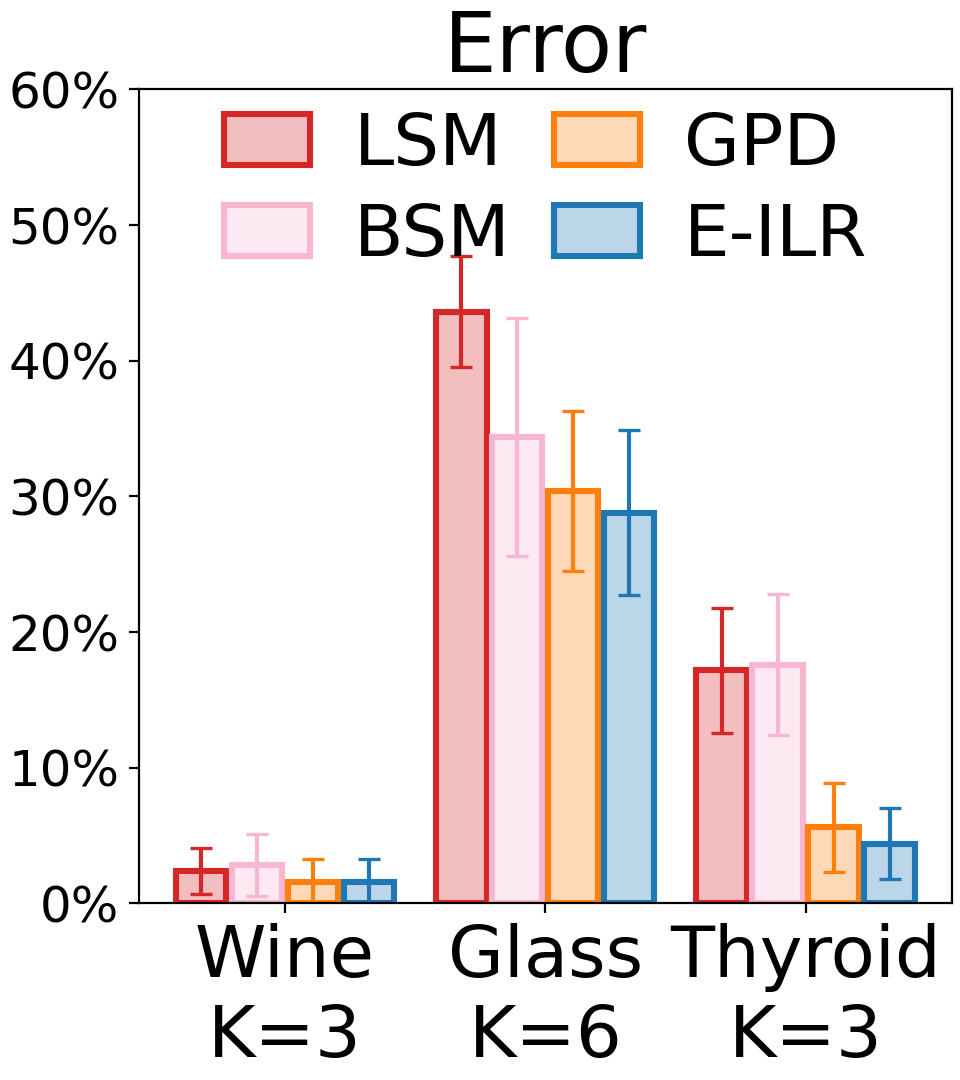
\includegraphics[width=0.3\linewidth]{figs/paper4/uci_conjugate/uci_best_conjugate_per_seed_error.png}
    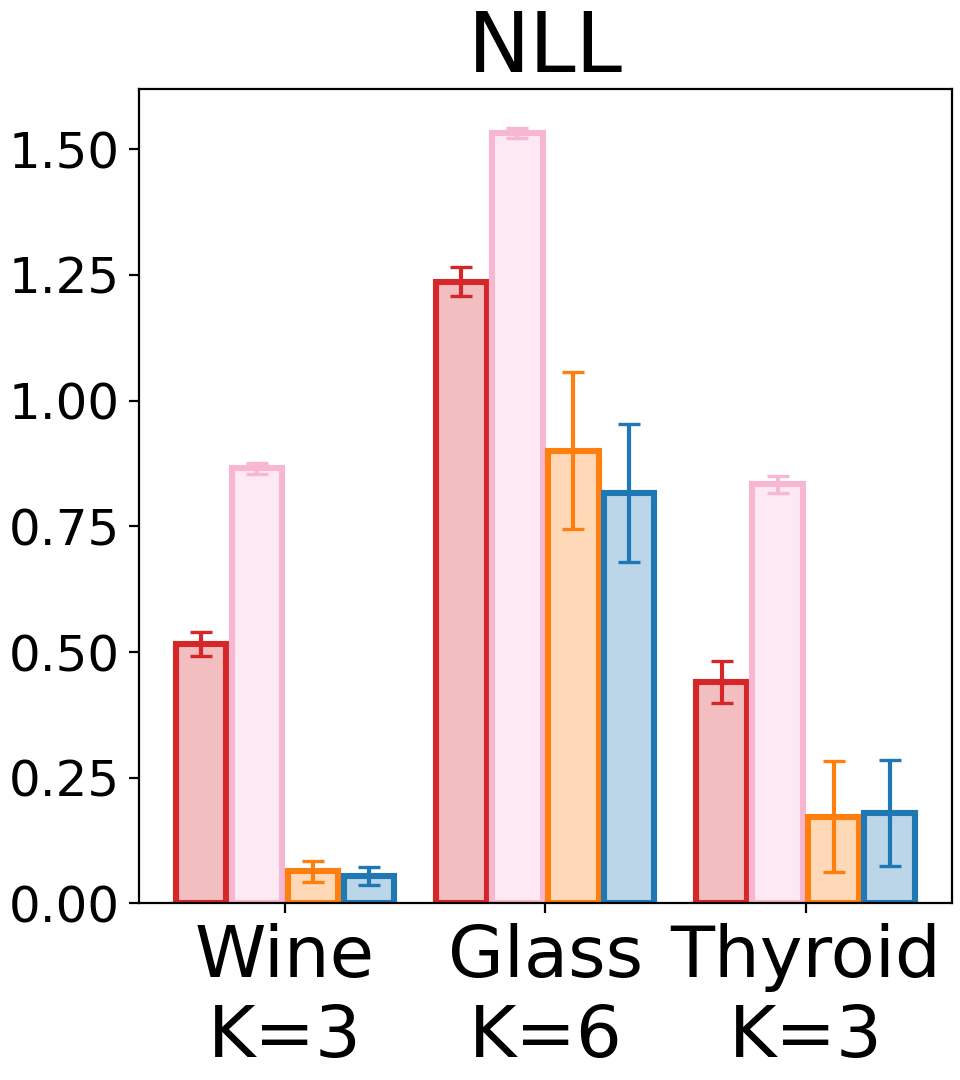
\includegraphics[width=0.3\linewidth]{figs/paper4/uci_conjugate/uci_best_conjugate_per_seed_nll.png}
    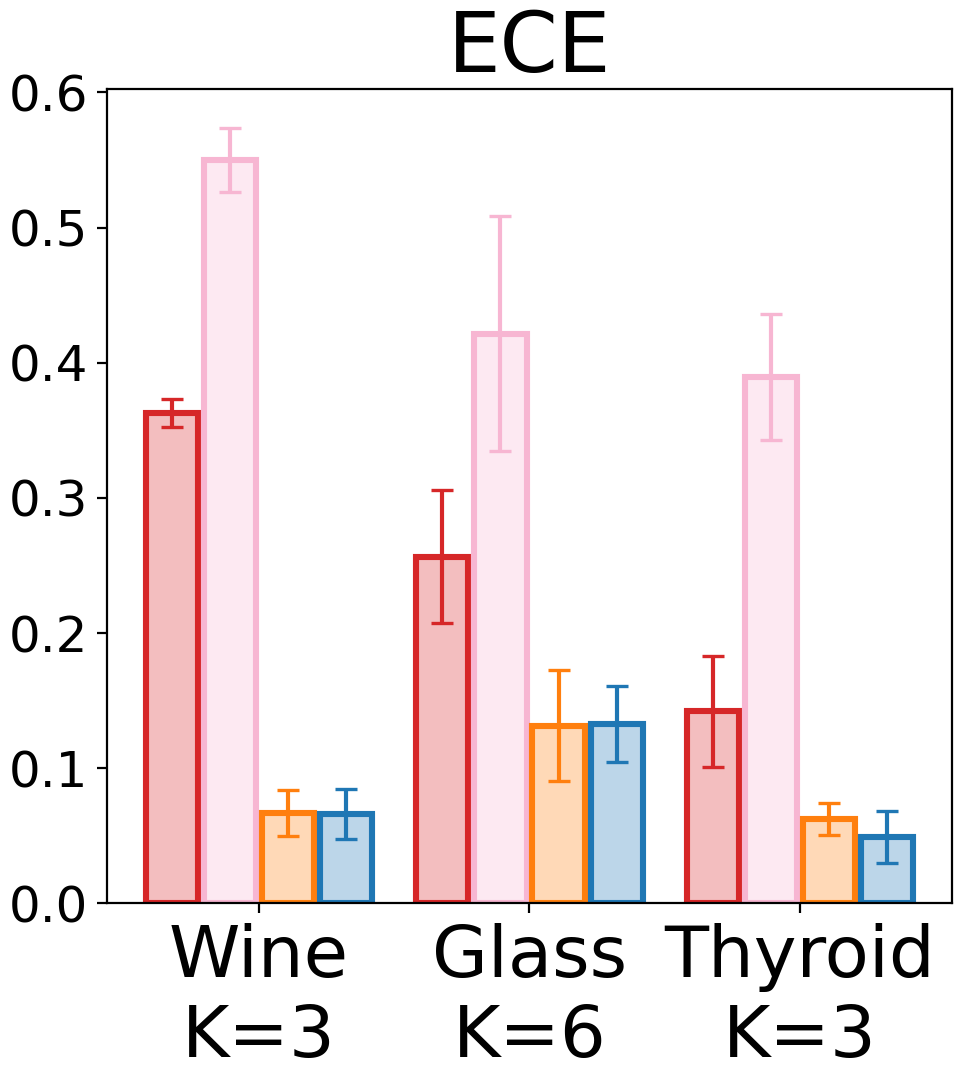
\includegraphics[width=0.3\linewidth]{figs/paper4/uci_conjugate/uci_best_conjugate_per_seed_ece.png}
    \caption{Error, NLL and ECE for UCI datasets in the exact setting.  }
    \label{fig:uci_conjugate}
\end{figure}

\paragraph{Sparse UCI regression}
We next consider seven larger UCI classification benchmarks, where inducing-point approximations are required. Figure~\ref{fig:uci_sparse} summarizes the results. Overall, Collapsed-ILR and sparse Dirichlet GP classification are the strongest methods across the three metrics. The two ILR-based sparse models are competitive with sparse GPD and are often slightly better calibrated. In particular, the ILR-based sparse methods obtain lower ECE on several tasks, and on the \textsc{Letter} data set Uncollapsed-ILR performs better than Collapsed-ILR. The data-augmented softmax baselines struggle here, especially as the number of classes increases. The main conclusion is that the sparse ILR constructions preserve the good calibration of the exact model while scaling to larger problems.


\begin{figure}
    \centering
    \begin{subfigure}[b]{0.7\linewidth}
        \centering
        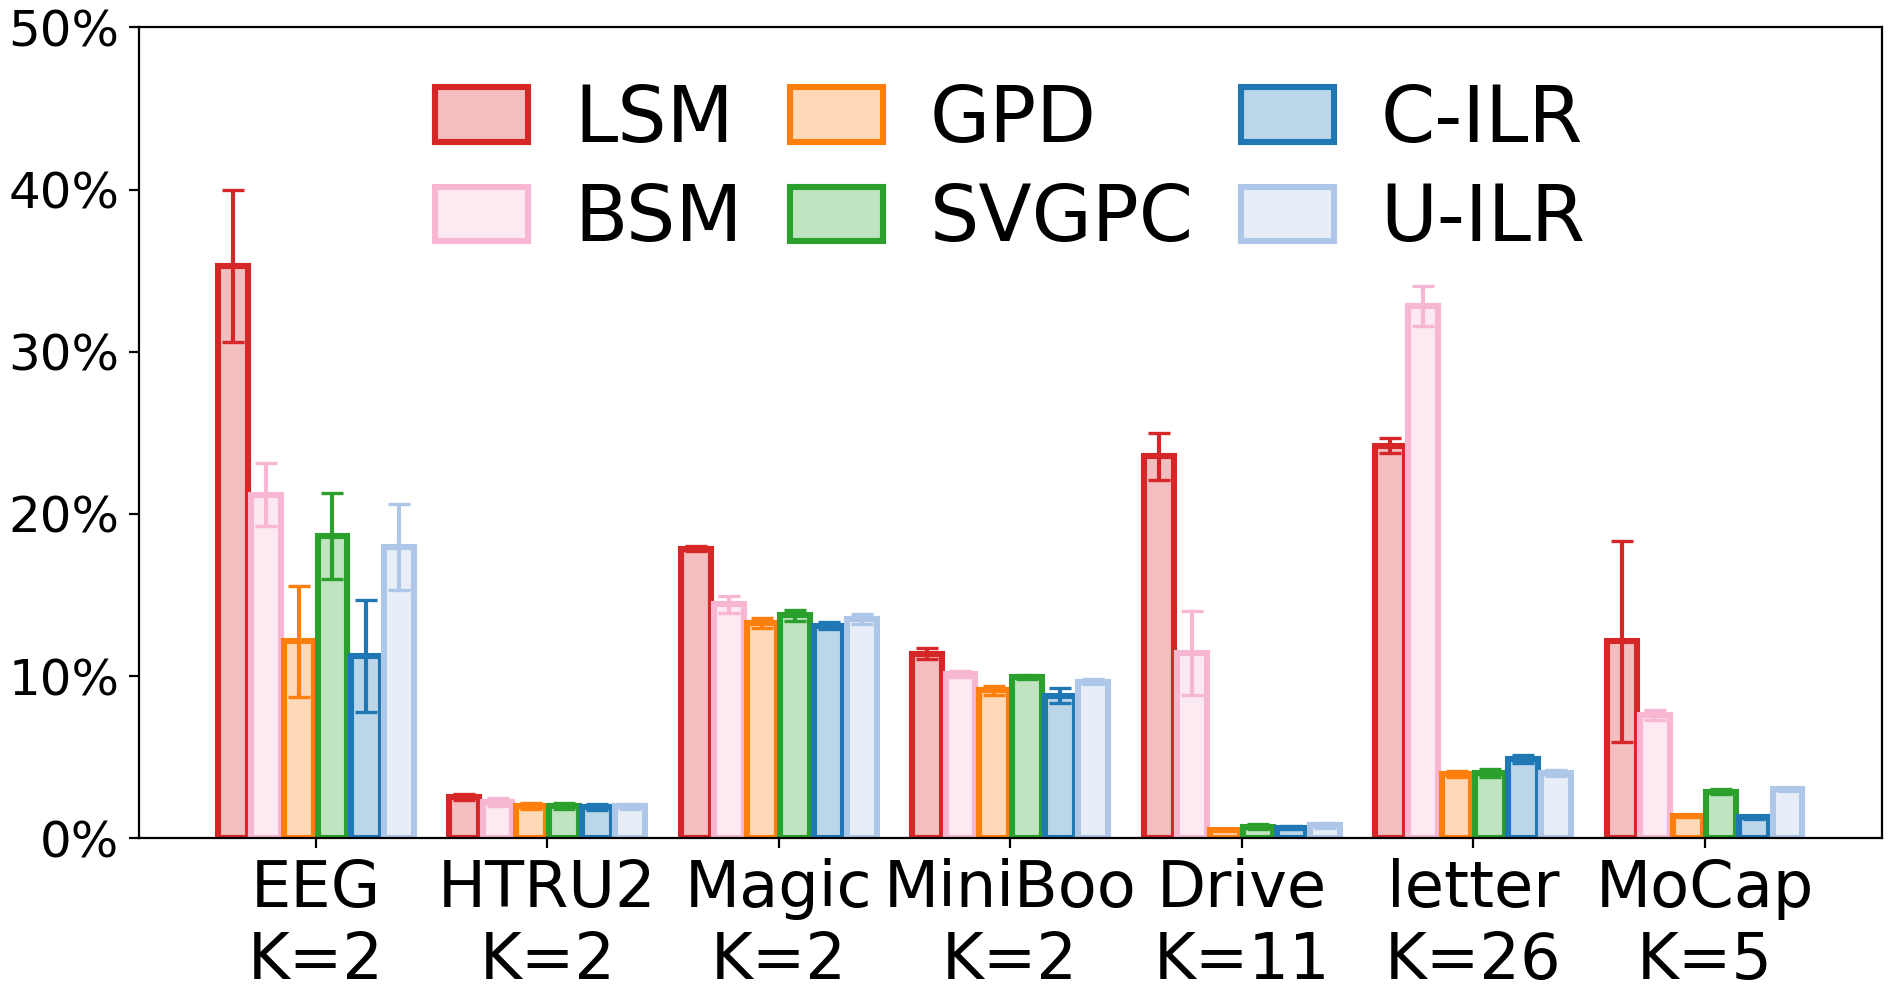
\includegraphics[width=\linewidth]{figs/paper4/uci_sparse/uci_best_sparse_per_seed_error.png}
        \caption{Error rate}
    \end{subfigure}
    \begin{subfigure}[b]{0.7\linewidth}
        \centering
        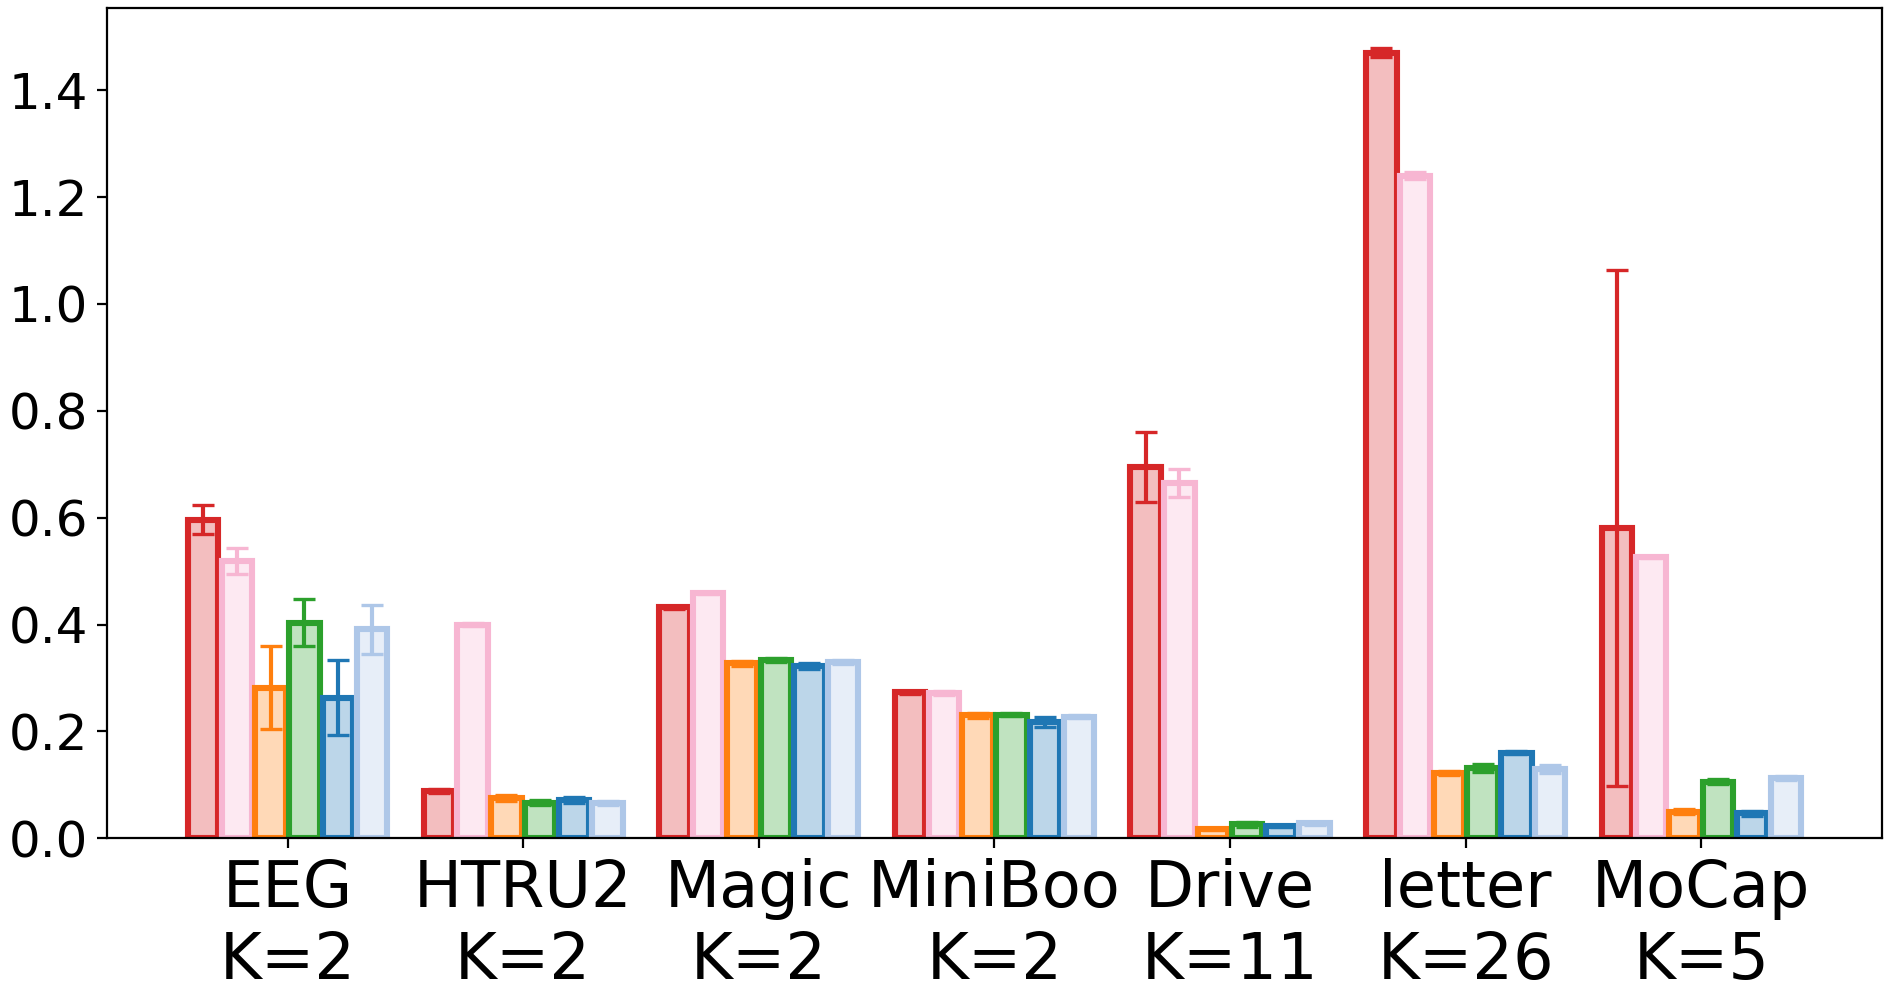
\includegraphics[width=\linewidth]{figs/paper4/uci_sparse/uci_best_sparse_per_seed_nll.png}
        \caption{NLL}
    \end{subfigure}
    \begin{subfigure}[b]{0.7\linewidth}
        \centering
        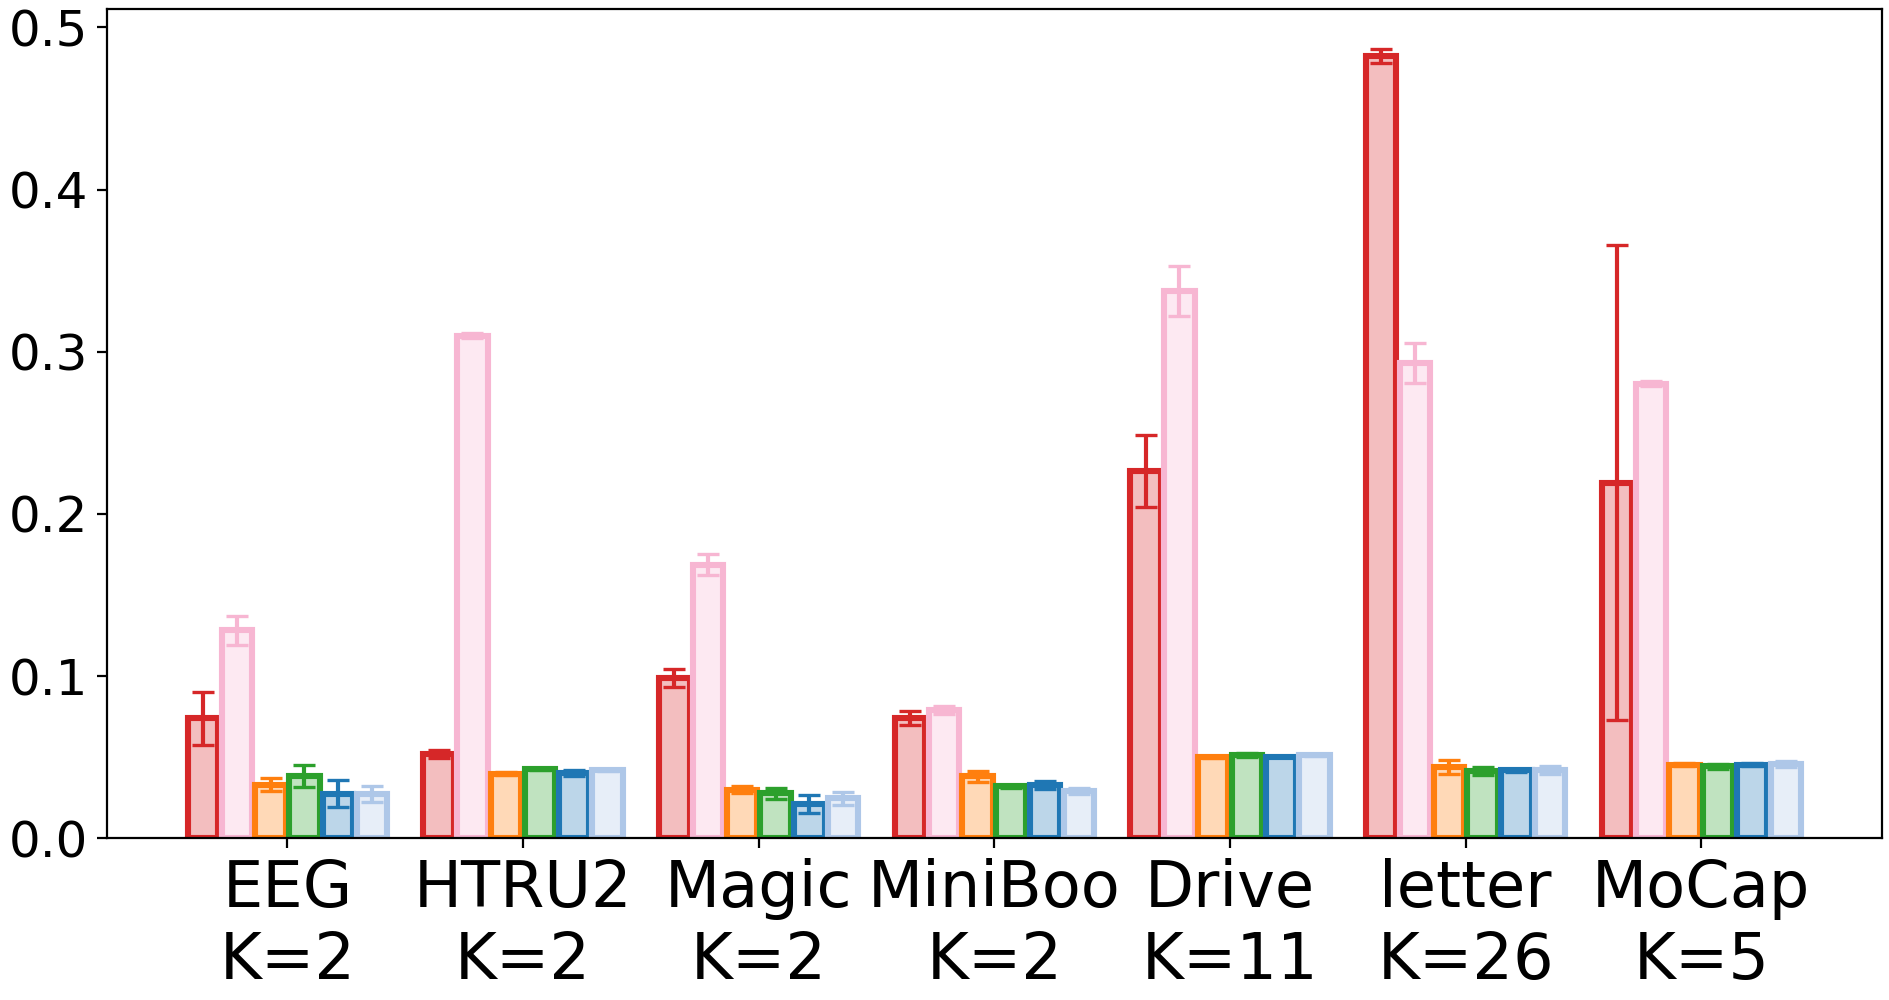
\includegraphics[width=\linewidth]{figs/paper4/uci_sparse/uci_best_sparse_per_seed_ece.png}
        \caption{ECE}
    \end{subfigure}    
    \caption{Sparse models performance on UCI datasets.  }
    \label{fig:uci_sparse}
\end{figure}
